\documentclass[10pt, a4paper]{article}
\usepackage[left=3.17cm, right=3.17cm, top=2.54cm, bottom=2.54cm]{geometry}
\usepackage[UTF8]{ctex}
\usepackage{amsmath}
\usepackage{amsfonts}
\usepackage{amssymb}
\usepackage{mathrsfs}
\usepackage{enumerate}
\usepackage{caption}
\usepackage{graphicx}
\usepackage{subfig}
\usepackage{siunitx}
\usepackage{minted}
\usemintedstyle{rainbow_dash}
% \usepackage{fontspec}
\setmonofont[]{Fira Code}
\usepackage{hyperref}
\hypersetup{unicode, colorlinks=true, linkcolor=black, urlcolor=blue}

\begin{document}
\definecolor{bg}{rgb}{0.95,0.95,0.95}

\title{Matlab\,语音处理实验报告}
\author{暮月}

\maketitle

\tableofcontents

\paragraph{环境与依赖说明}本次实验使用的是Matlab R2020a Update3,主要使用了XXX。Matlab设置为使用utf-8编码,所有代码文件无特殊情况均为此编码,注释以英文为主。

\section{语音预测模型}

\subsection{滤波器}\label{sec:filter}

对滤波器差分方程做Z变换:

\begin{align*}
    e(n) & = s(n) - a_1 s(n - 1) - a_2 s(n - 2)       \\
    E(z) & = S(z) - a_1 z^{-1} S(z) - a_2 z^{-2} S(z)
\end{align*}

所以传递函数为:

\begin{align*}
    H(z) = \frac{S(z)}{E(z)} = \frac{1}{1 - a_1 z^{-1} - a_2 z^{-2}} = \frac{z^2}{z^2 - a_1 z - a_2}
\end{align*}

从而共振峰频率为:

\begin{align*}
    f & = \frac{\omega}{2\pi} = \frac{\Omega}{2\pi T} = \frac{|\angle{p_i}|}{2\pi T} \\
      & = \frac{\text{abs(angle($p_i$))}}{2\pi T}
\end{align*}

使用\mintinline{matlab}{roots([1, -1.3789, 0.9506])}求得两极点为$0.6895 + 0.6894i$和$0.6895 - 0.6894i$再代入上式得到分子$\Omega$为$0.7854$rad,即$0.25\pi$rad。根据说明,取采样间隔为10ms80样本点,即0.125ms,从而得到$f = \frac{0.7854\text{rad}}{2\pi \cdot 0.125\text{ms}} = 1000.00\text{Hz}$。

使用\mintinline{matlab}{zplane}、\mintinline{matlab}{freqz}、\mintinline{matlab}{impz}和\mintinline{matlab}{filter}得到相关图像。

\begin{figure}[h]
    \centering
    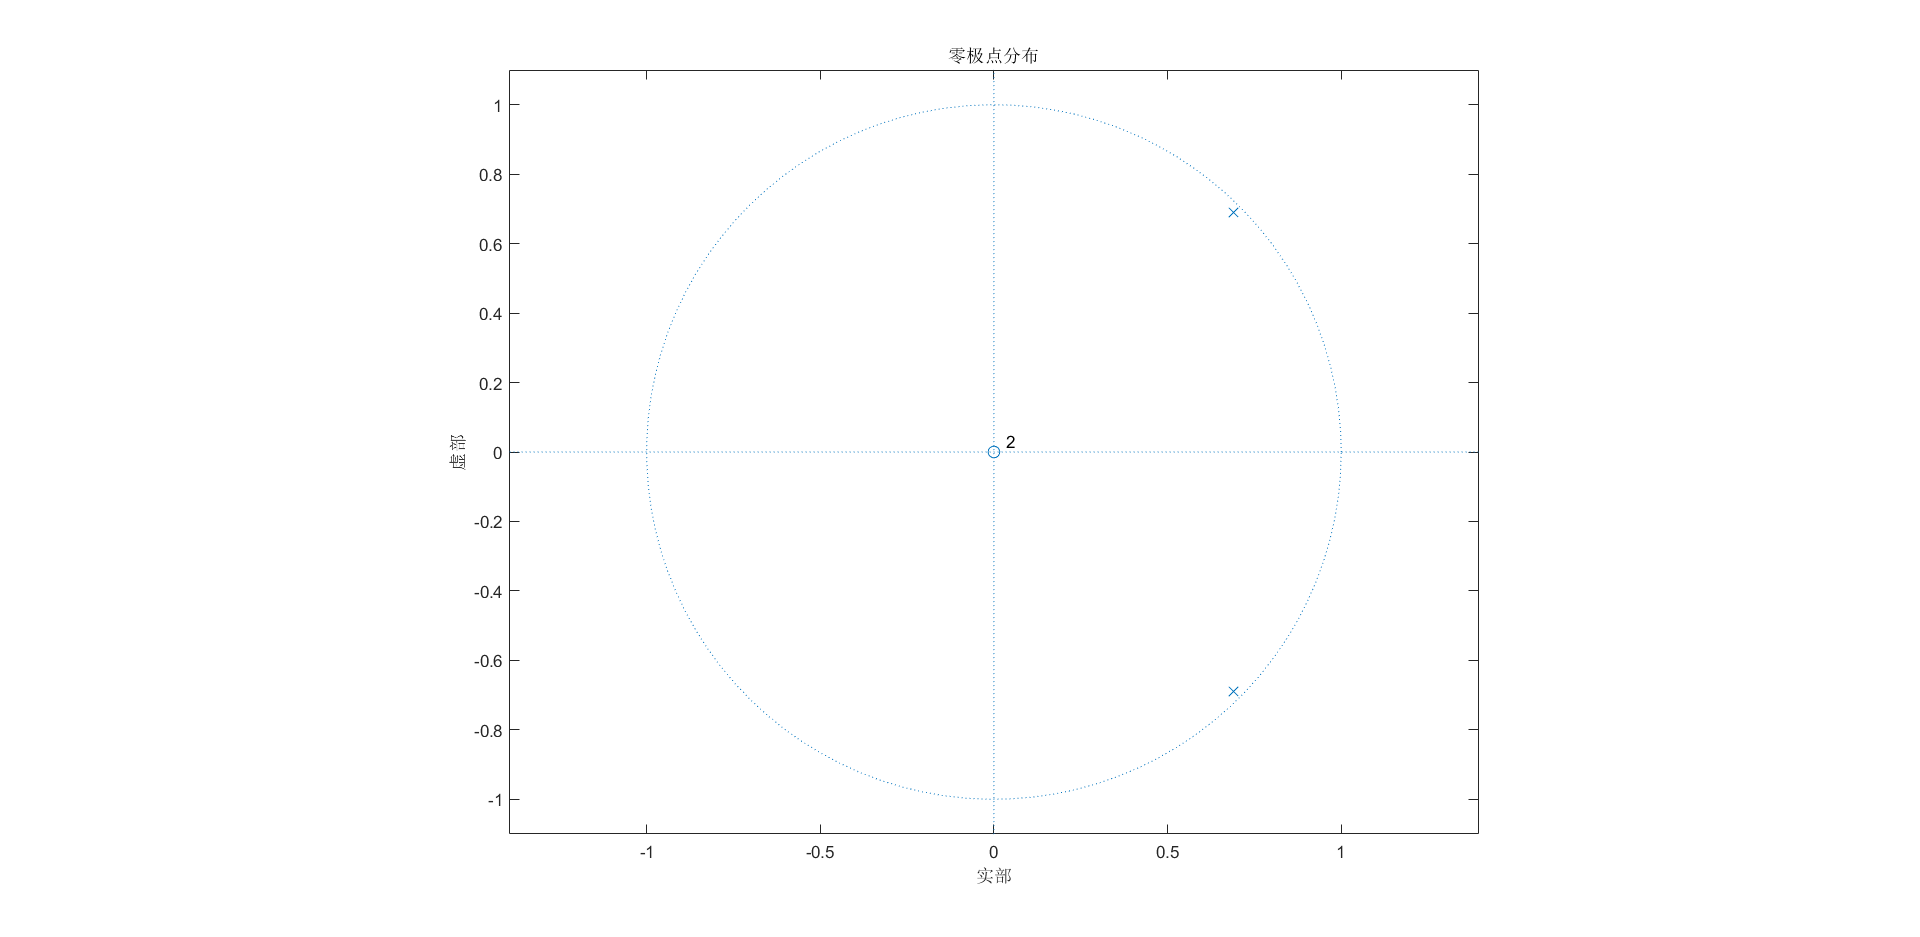
\includegraphics[width=.8\textwidth]{../assets/1_1_zplane.png}
    \caption{滤波器的零极点分布}
    \label{fig:exp1_1_zplane}
\end{figure}

\begin{figure}[h]
    \centering
    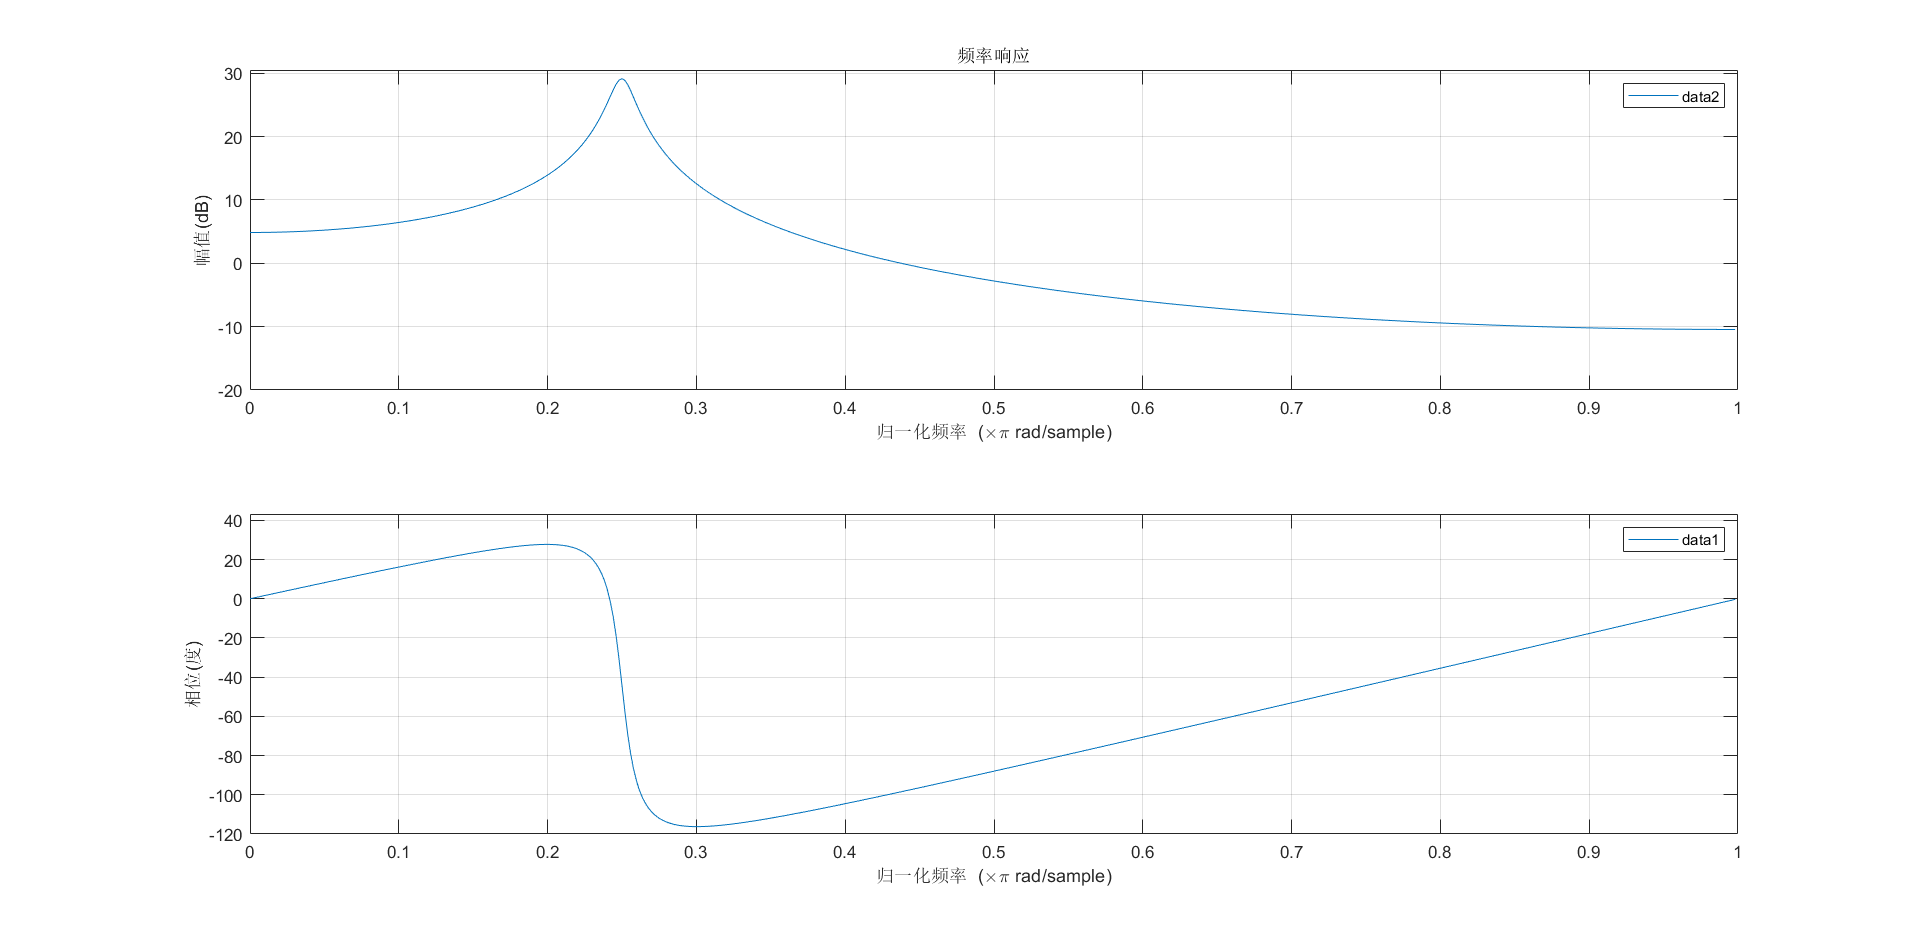
\includegraphics[width=.8\textwidth]{../assets/1_1_freqz.png}
    \caption{滤波器的频率响应}
    \label{fig:exp1_1_freqz}
\end{figure}

\begin{figure}[!ht]
    \centering
    \subfloat[impz]{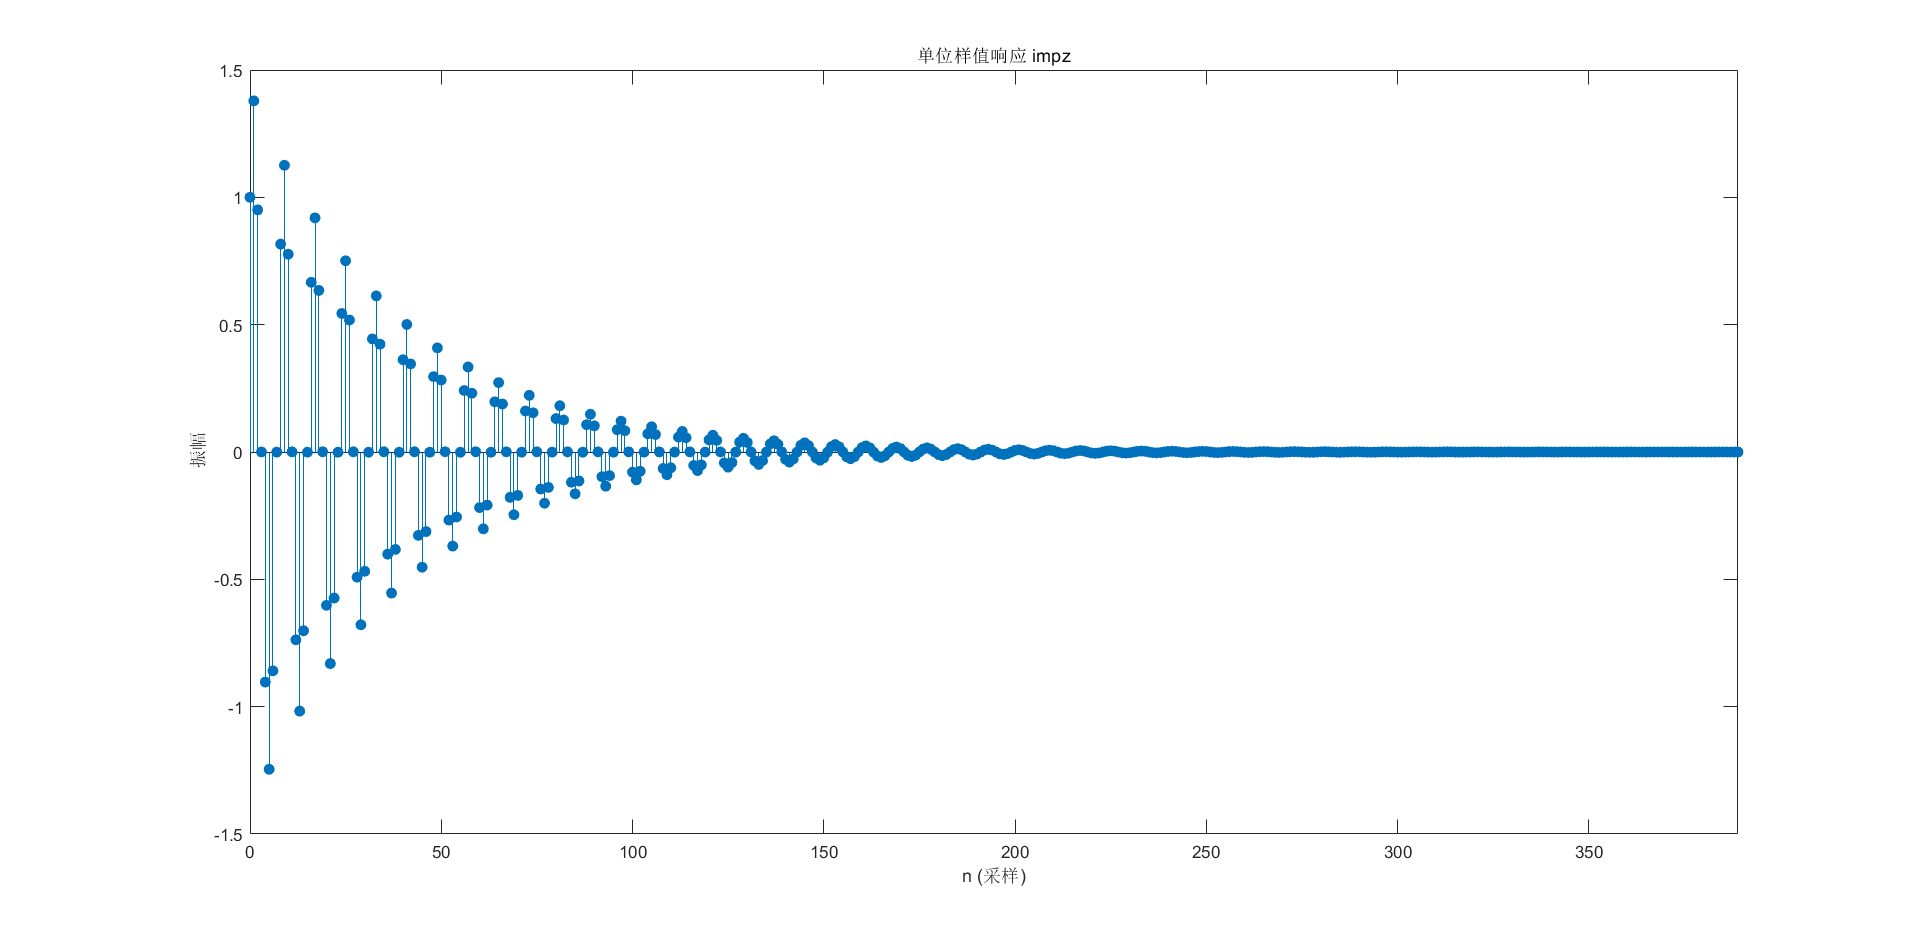
\includegraphics[width=.4\textwidth]{../assets/1_1_impz.png}}
    \subfloat[filter]{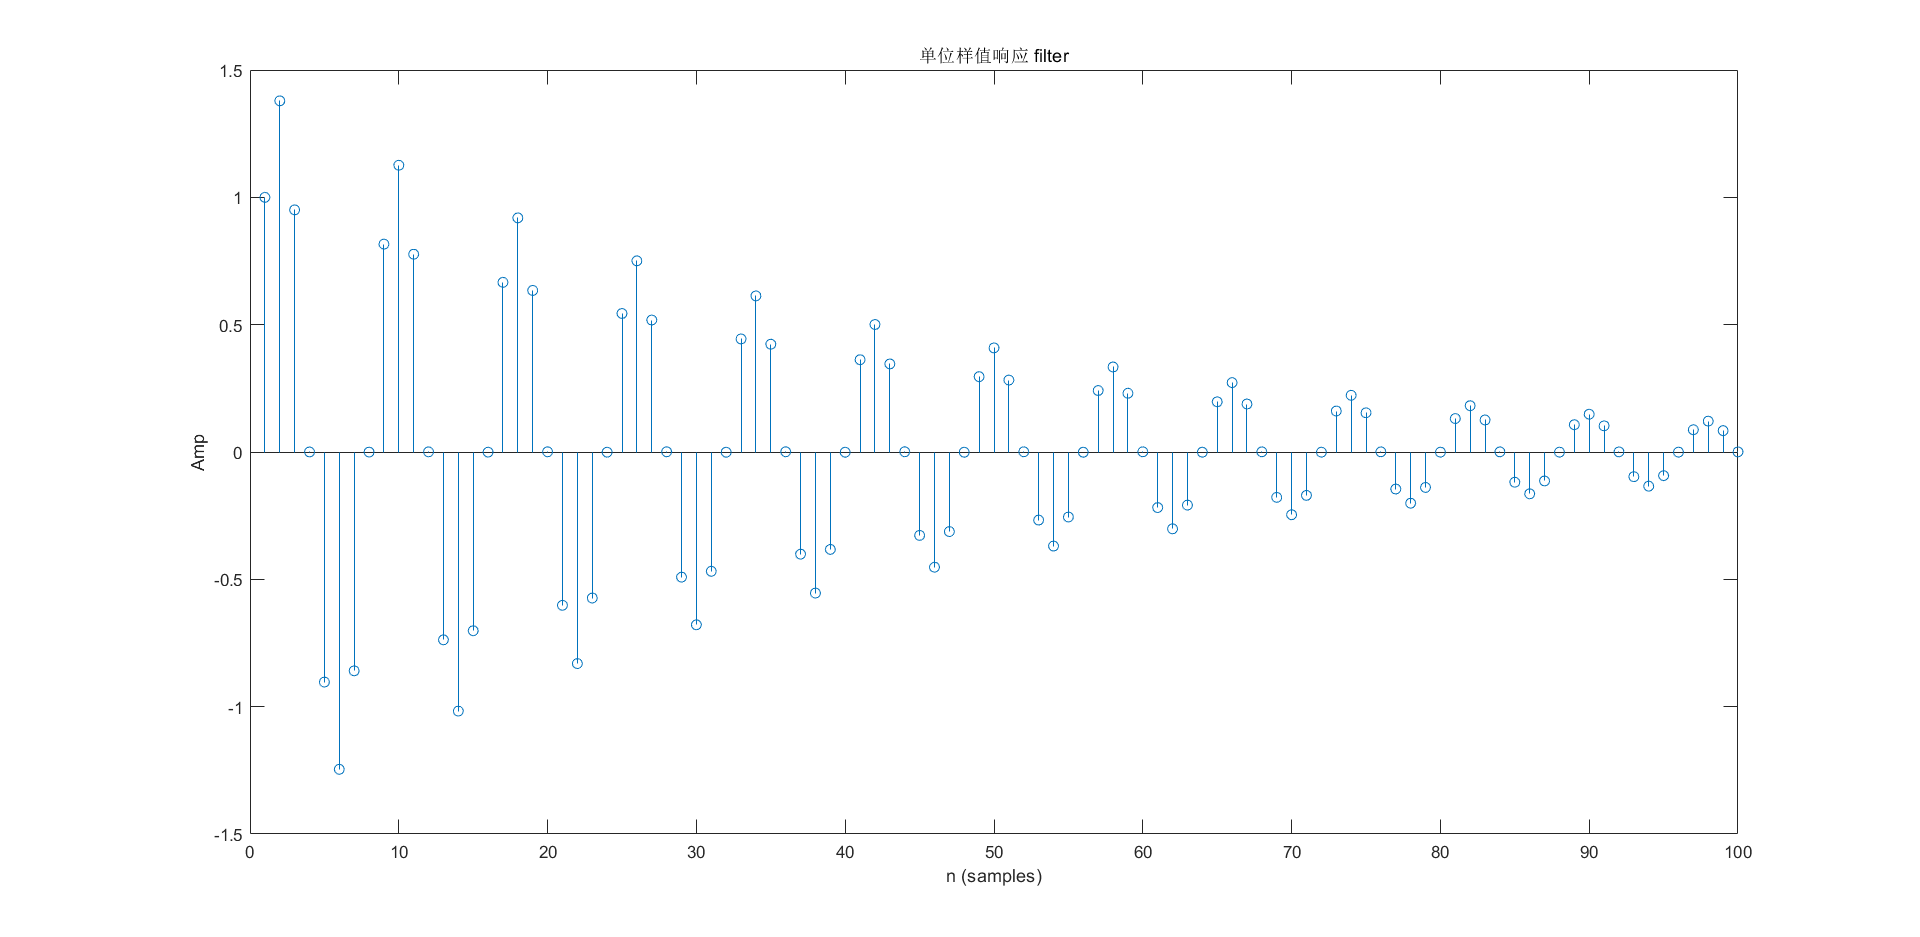
\includegraphics[width=.4\textwidth]{../assets/1_1_filter.png}}
    \caption{滤波器的单位样值响应}
    \label{fig:exp1_1_impz}
\end{figure}

如图\ref{fig:exp1_1_zplane},该滤波器在原点处有一二阶零点,在$\pm\frac{\pi}{4}$靠近单位圆2处有一对共轭一阶极点。如图\ref{fig:exp1_1_freqz},该滤波器在$0.25\pi$rad处(即上方计算的共振峰频率处)有共振峰,同时相位为0。

该滤波器的单位样值响应如图\ref{fig:exp1_1_impz}。这里由于\mintinline{matlab}{filter}的参数只取了100个采样点,而不是\mintinline{matlab}{impz}\\默认生成的400个采样点,故结果比较稀疏。实际上,两个函数得到的结果完全一致。

\subsection{\texttt{speechproc}的基本流程}

\mintinline{matlab}{speechproc}读取一段音频,对其进行一系列处理后保存处理结果,并将控制权交还调用脚本。流程如下:

\begin{enumerate}
    \item 定义常数:帧长、窗长、预测系数个数、音频文件
    \item 载入语音,并计算相关参数,定义合成信号与滤波器状态等变量
    \item 循环处理每帧语音
          \begin{enumerate}
              \item 计算预测系数
              \item 27帧时,显示预测系统的零极点分布图
              \item 使用\mintinline{matlab}{filter}计算本帧语音\mintinline{matlab}{s_f}的激励,存入\mintinline{matlab}{exc}
              \item 使用\mintinline{matlab}{filter}和\mintinline{matlab}{exc}重建语音,存入\mintinline{matlab}{s_rec}
              \item 计算基音周期\mintinline{matlab}{PT}、合成激励的能量\mintinline{matlab}{G}
              \item 生成合成激励\mintinline{matlab}{exc_syn},并合成语音\mintinline{matlab}{s_syn}
              \item 将合成激励的长度增加一倍,合成语音\mintinline{matlab}{s_syn_v}
              \item 将基音周期减小一半,将共振峰频率增加150Hz,合成语音\mintinline{matlab}{s_syn_t}
          \end{enumerate}
    \item 试听语音
    \item 保存语音与激励
\end{enumerate}

\subsection{预测系统的零极点分布}

预测模型为:

\begin{align*}
    e(n) = s(n) - \sum_{k=1}^N a_k s(n - k)
\end{align*}

注意到这里的输入是$s(n)$,输出是残差$e(n)$。故只需将等式右边的系数作为\mintinline{matlab}{zplane}的第一项系数便可以得到预测系统的零极点分布图。添加如下代码:

\begin{minted}[bgcolor=bg]{matlab}
if n == 27
% (3) 在此位置写程序,观察预测系统的零极点图
    figure;
    zplane(A, 1);
    title('预测系统的零极点分布图');
end
\end{minted}

\begin{figure}[h]
    \centering
    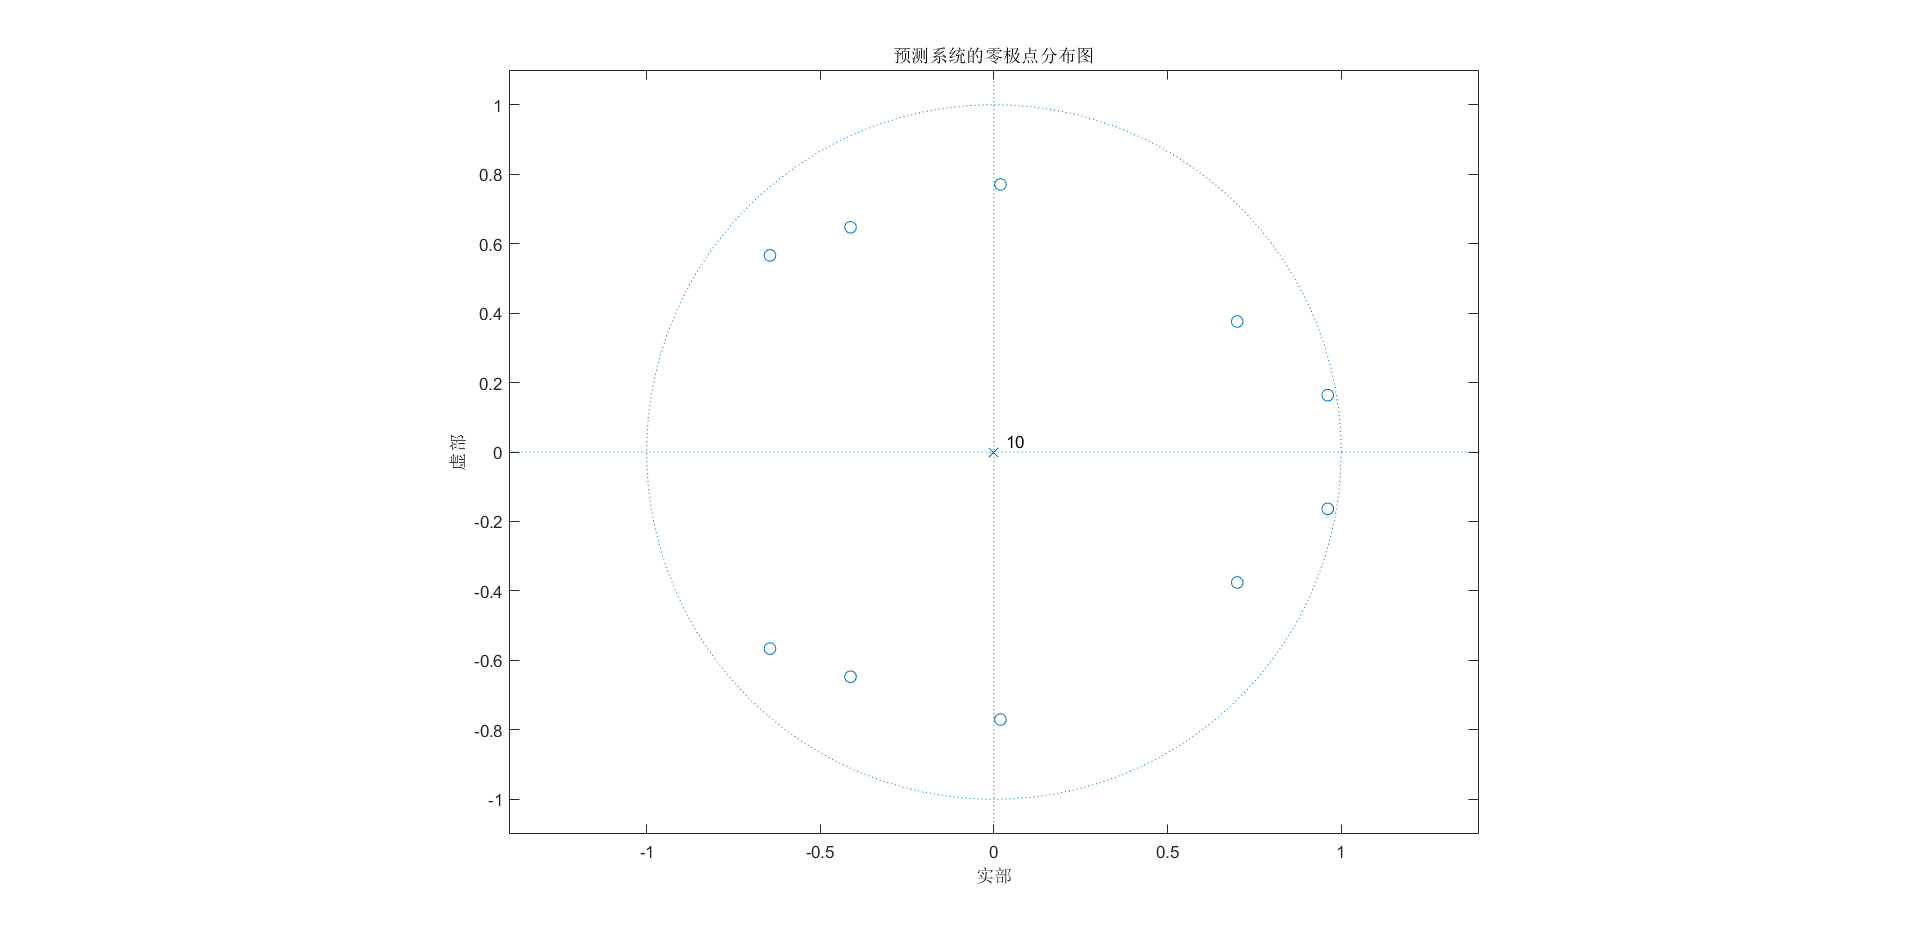
\includegraphics[width=.8\textwidth]{../assets/1_3_zplane.png}
    \caption{预测系统的零极点分布图}
    \label{fig:1_3_zplane}
\end{figure}

可以看到,27帧时的预测模型有一个10阶极点和五对共轭零点。由于其为声道模型的逆系统,此时的声道模型应有一个10阶零点和五对共轭极点。

\subsection{用\texttt{filter}计算激励}

根据Matlab文档,\mintinline{matlab}{[y, zf] = filter(b, a, x, zi)}接受系统的分子b、分母a、输入x、滤波器延迟初始条件zi,返回输出y和延迟最终条件zf。因而使用如下代码存储激励和滤波器状态:

\begin{minted}[bgcolor=bg]{matlab}
[exc((n - 1) * FL + 1 : n * FL), zi_pre] = ...
    filter(A, 1, s_f, zi_pre);
\end{minted}

\subsection{用\texttt{filter}和\texttt{exc}重建语音}

与上一节类似,注意重建语音与预测模型的零极点交换,故使用如下代码存储重建的语音和滤波器状态:

\begin{minted}[bgcolor=bg]{matlab}
[s_rec((n - 1) * FL + 1 : n * FL), zi_rec] = ...
    filter(1, A, exc((n - 1) * FL + 1 : n * FL), zi_rec);
\end{minted}

\subsection{语音、激励、重建语音的区别}

阅读Matlab关于音频部分的文档,注意到\mintinline{matlab}{sound}接受的第一个参数音频为$[-1, 1]$间实数组成的向量。故应将从voice.pcm读入的语音进行量化后使用。

使用Matlab确认语音向量的值为16位符号数,故除以32768进行量化,再使用\mintinline{matlab}{sound},以采样频率8000Hz进行播放。代码如下:

\begin{minted}[bgcolor=bg]{matlab}
sound([s; exc; s_rec] / 32768, 8000);
\end{minted}

再使用\mintinline{matlab}{plot}绘制波形,并仿照Matlab关于\mintinline{matlab}{fft}的文档生成并绘制语音、激励、重建语音的频域图形。

\begin{figure}[h]
    \centering
    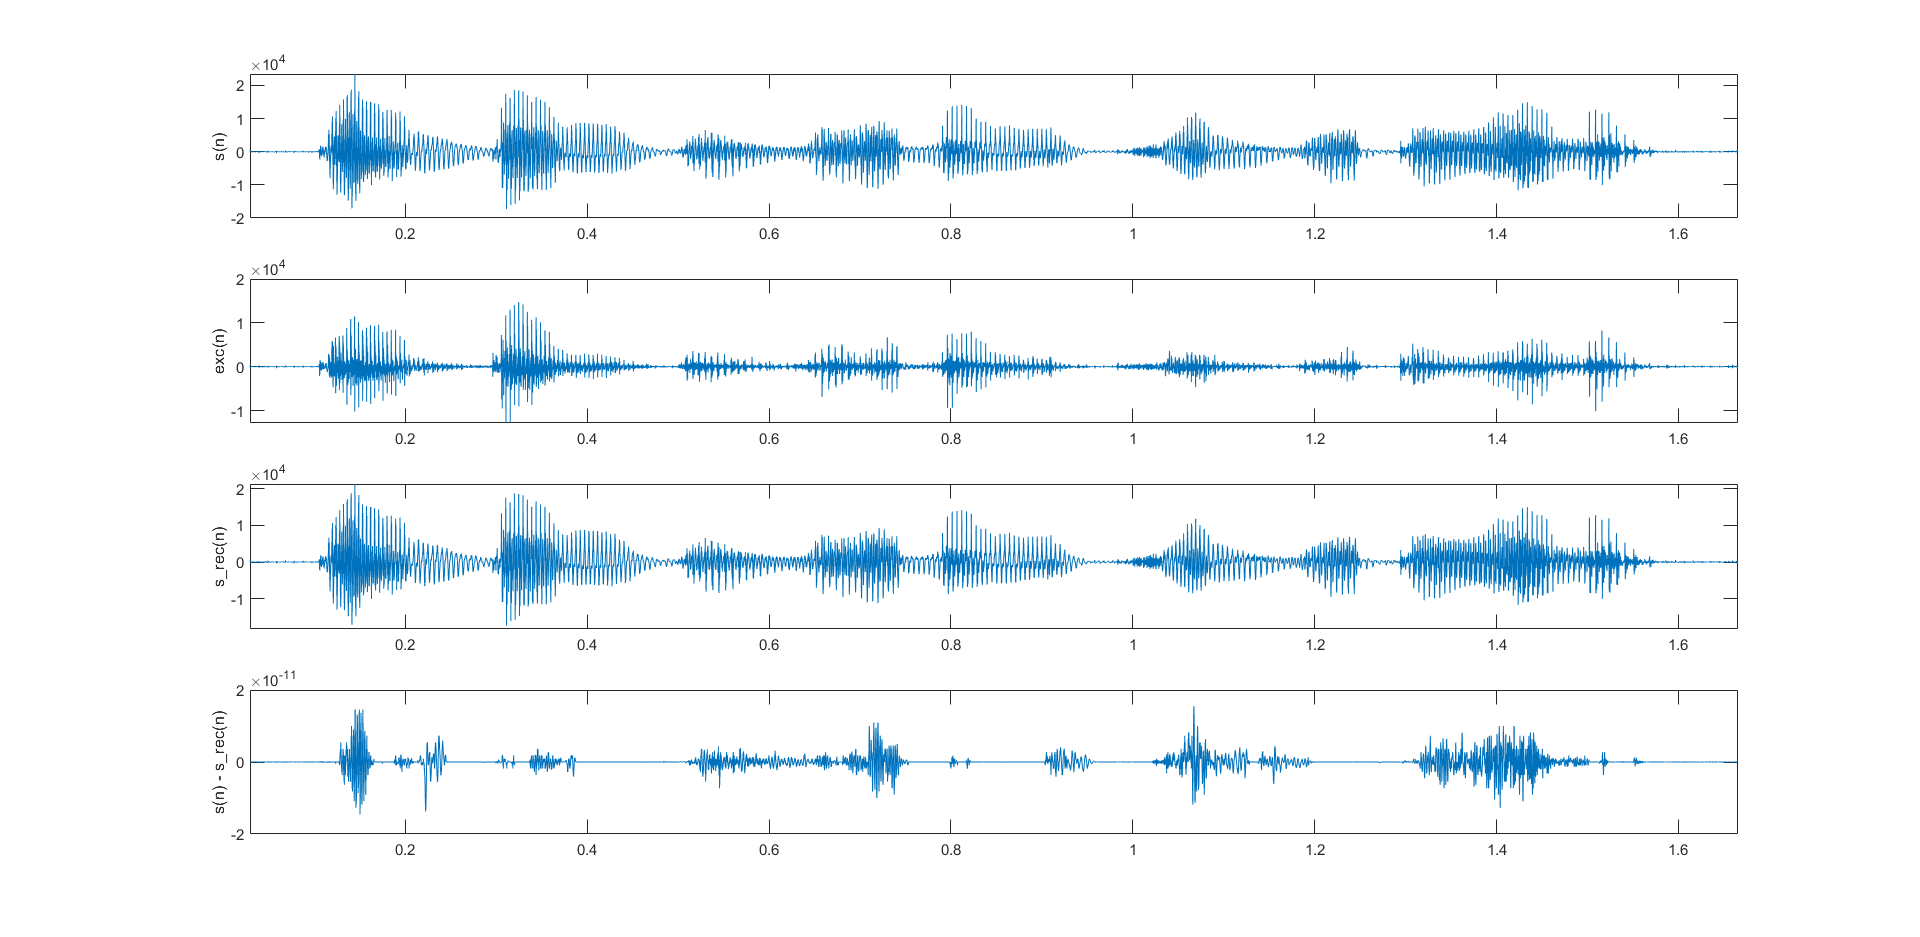
\includegraphics[width=.95\textwidth]{../assets/1_6_time.png}
    \caption{语音、激励、重建语音时域}
    \label{fig:1_6_time}
\end{figure}

\begin{figure}[h]
    \centering
    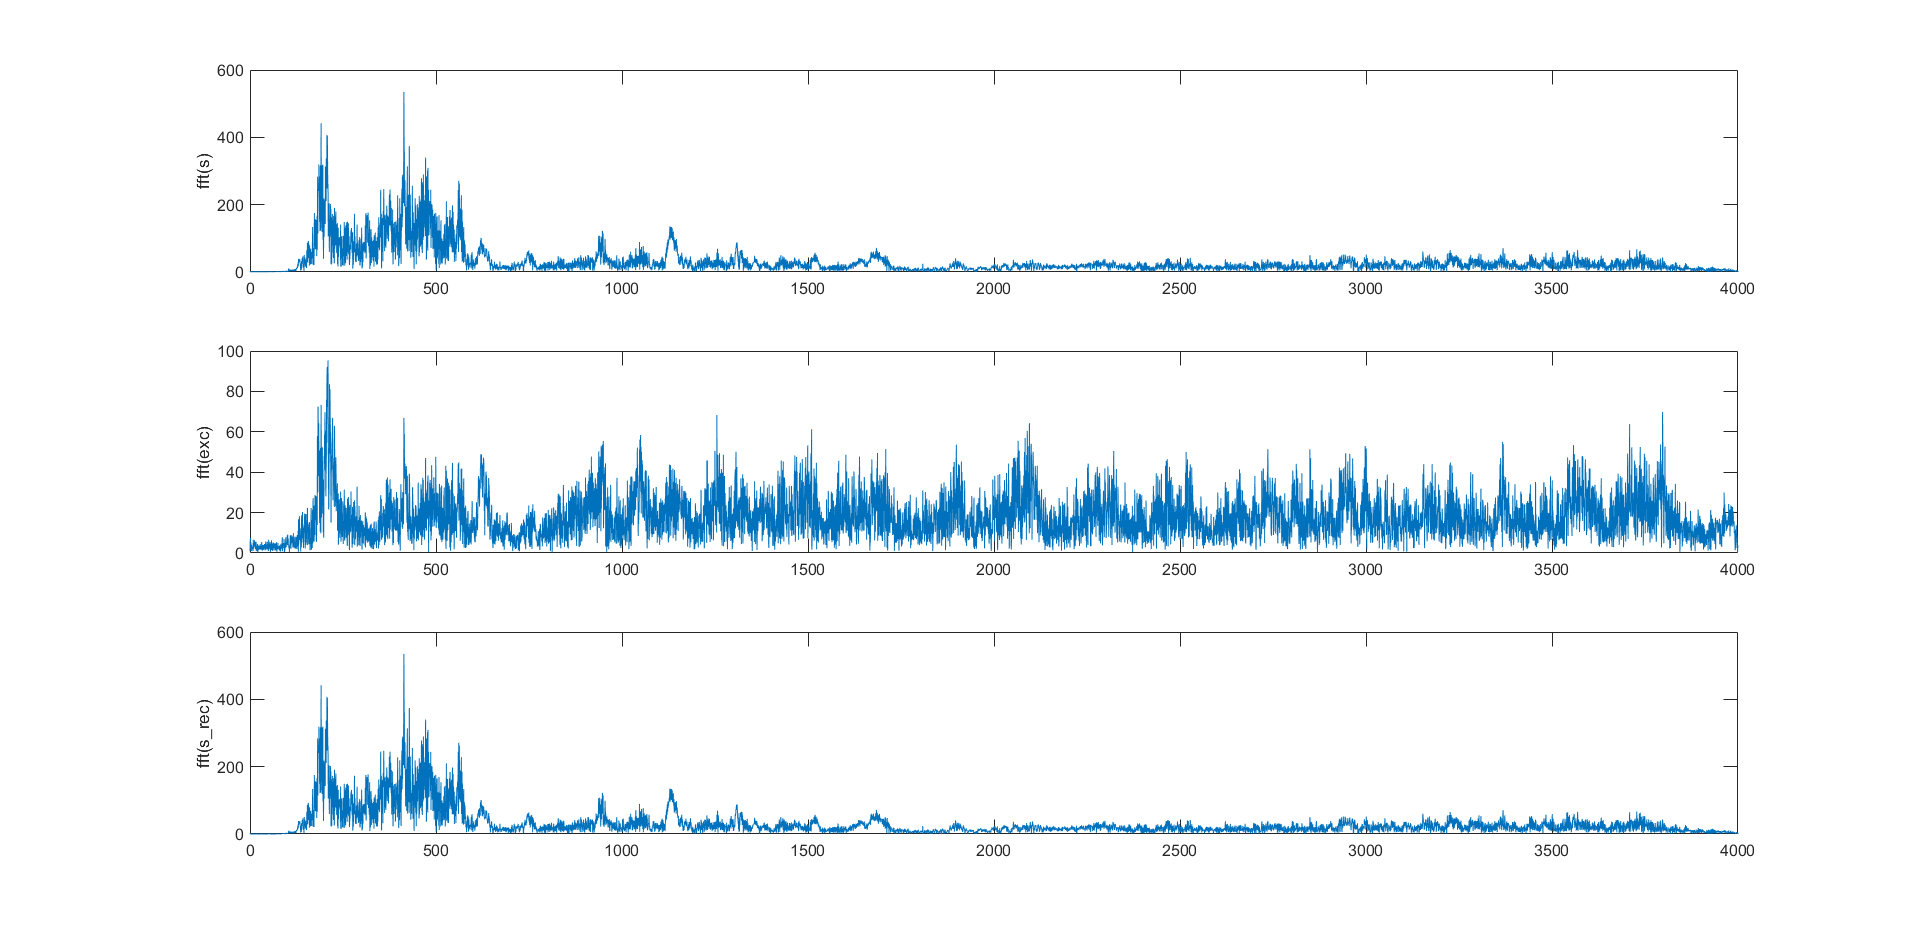
\includegraphics[width=.95\textwidth]{../assets/1_6_freq.png}
    \caption{语音、激励、重建语音频域}
    \label{fig:1_6_freq}
\end{figure}

观察图\ref{fig:1_6_time}中的波形,语音和重建语音几乎没有什么区别,差值普遍在$10^{-11}$以下。转换到频域(图\ref{fig:1_6_freq})后,语音和重建语音肉眼难见区别,相比之下激励各频段的幅度基本一致,没有语音明显的低频分量占比大的现象。使用\mintinline{matlab}{sound}播放出的声音,语音和重建语音听不出什么区别,而激励会有较多杂音,听上去有老旧收音机的感觉且声音较小,应是频域图中较多的高频分量而普遍较小的幅度导致。

使用\mintinline{matlab}{linkaxes}将语音、激励、重建语音的刻度同步,放大后截取一小段波形如图\ref{fig:1_6_time_local}。可以看出,激励因为有更多的高频分量,变化更为频繁,这与前面分析一致。语音和重建语音仍然肉眼难见明显区别。

\begin{figure}[h]
    \centering
    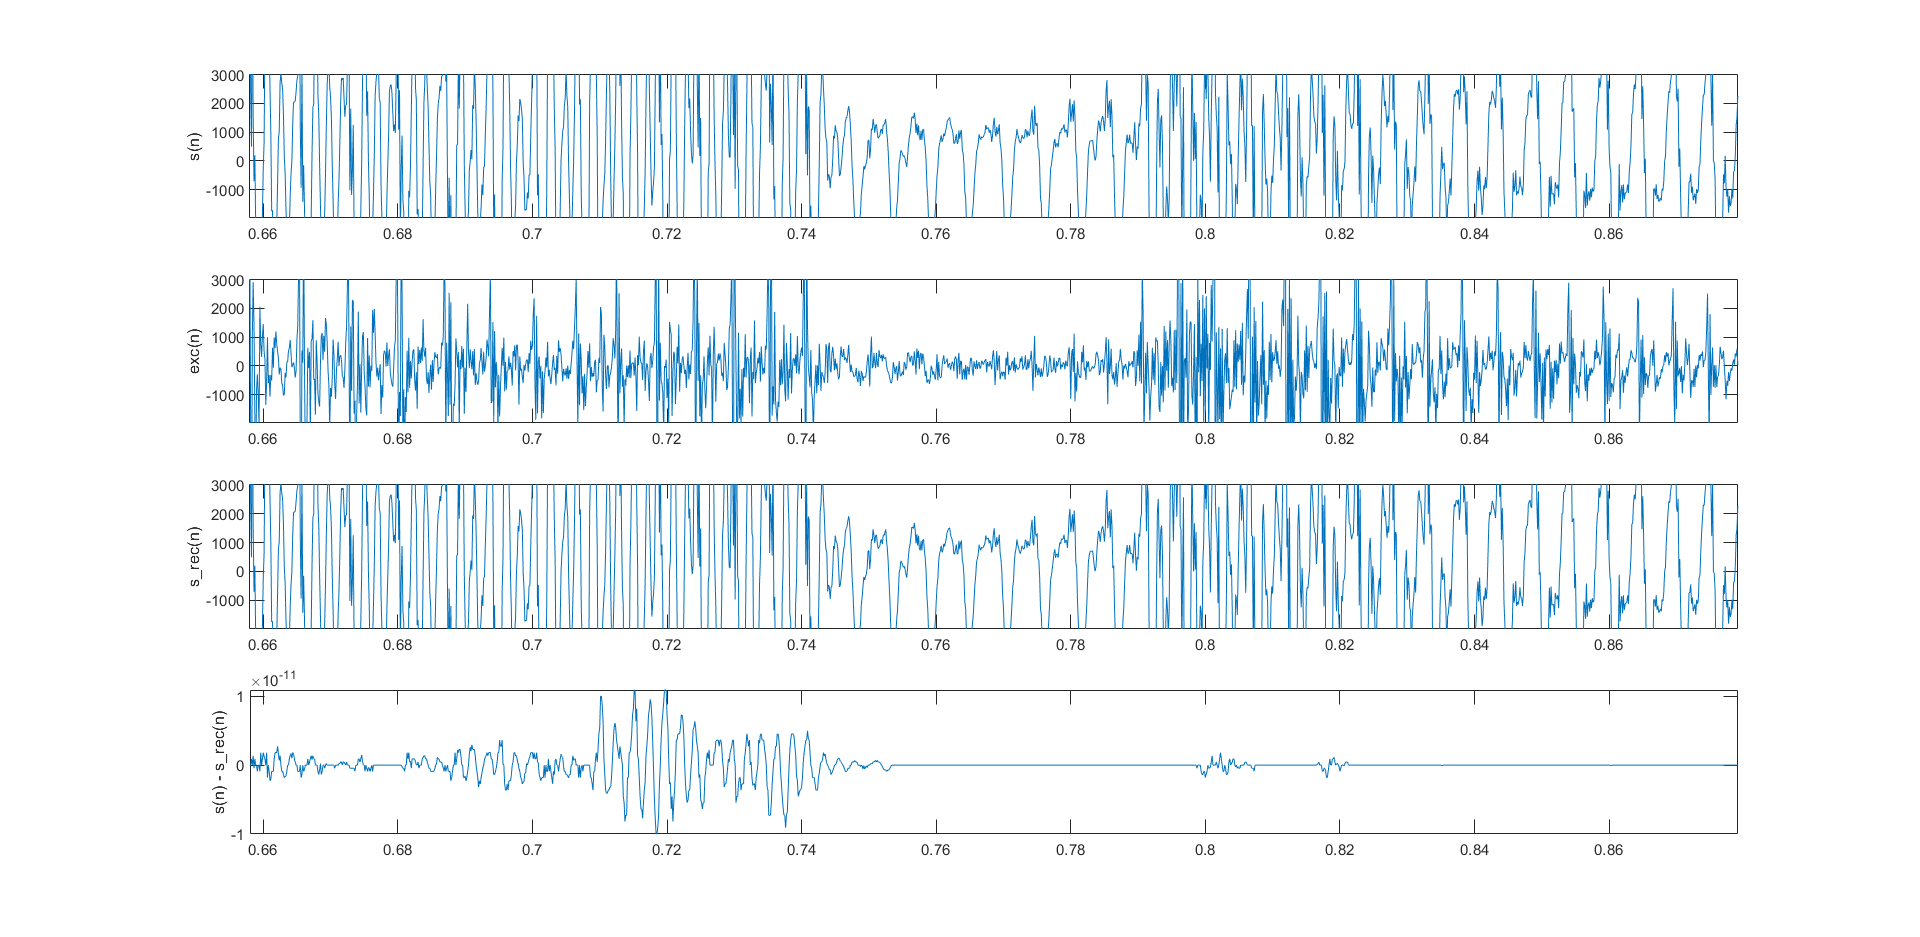
\includegraphics[width=.95\textwidth]{../assets/1_6_time_local.png}
    \caption{语音、激励、重建语音时域局部}
    \label{fig:1_6_time_local}
\end{figure}

\section{语音合成模型}

\subsection{基音周期固定的单位样值串}\label{sec:pitch_period_fixed}

单位样值串由下式定义:

\begin{align*}
    x(n) = \sum_{i = 0}^{NS - 1} \delta(n - iN)
\end{align*}

由采样率8kHz,单位样值串200Hz,计算得:

\begin{align*}
    N  & = \frac{F_s}{f} = \frac{8000}{200} = 40 \\
    NS & = f \cdot t = 200 \times 1 = 200
\end{align*}

可以使用如下函数实现单位样值串的生成:

\begin{minted}[bgcolor=bg]{matlab}
function signal = unit_samples(sample_freq, freq, duration)
signal = zeros(1, round(sample_freq * duration));
NS = round(freq * duration);
N = round(sample_freq / freq);

i = 0 : NS - 1;
signal(i * N + 1) = 1;
end
\end{minted}

听起来300Hz的单位样值串音调更高,同时播放时是协和的。使用音调矫正器具测量得到,200Hz约为$G_3^\#$,300Hz约为$D_4^\#$,正好相差纯五度,同时播放为协和的和声。


\subsection{基音周期变化的信号}\label{sec:pitch_period_change}

使用循环实现较为简单,代码如下:

\begin{minted}[bgcolor=bg]{matlab}
function signal = varied_unit_samples(sample_freq, duration)

sig_len = round(sample_freq * duration);

signal = zeros(1, sig_len);

pos = 1;
while pos <= sig_len
    signal(pos) = 1;
    m = ceil(pos / (0.01 * sample_freq));
    PT = 80 + 5 * mod(m, 50);
    pos = pos + PT;
end
end
\end{minted}

这样实现的问题是每个10ms的分界处PT会采用前一个10ms的值,不过影响较小,应不会对声音产生特别大的影响。另一种实现思路是先求得每一段对应的索引向量$[1, 1+PT, 1+2PT, \cdots]$,然后将这些索引向量拼接起来,再使用\mintinline{matlab}{signal(index_array) = 1}的形式产生信号。

使用下方代码产生一段10s的音频并播放:

\begin{minted}[bgcolor=bg]{matlab}
sig = varied_unit_samples(8000, 10);
sound(sig, 8000);
\end{minted}

这段音频听上去有较强的节奏感和粒子效果,比较接近于“电音”这类音乐的背景伴奏。

\subsection{将\ref{sec:pitch_period_change}中信号输入\ref{sec:filter}中滤波器}

使用下方代码生成并听音频:

\begin{minted}[bgcolor=bg]{matlab}
b = 1;
a = [1, -1.3789, 0.9506];
e = varied_unit_samples(8000, 5);

s = filter(b, a, e);
s = s / max(abs(s));

sound([e, s], 8000);
\end{minted}

听上去的感觉是滤波之后音调变低,相对不那么刺耳,有点像敲击木鱼和推拉老旧木门的声音。绘制时域和频域波形如图\ref{fig:2_3_time}和图\ref{fig:2_3_freq}。

\begin{figure}[h]
    \centering
    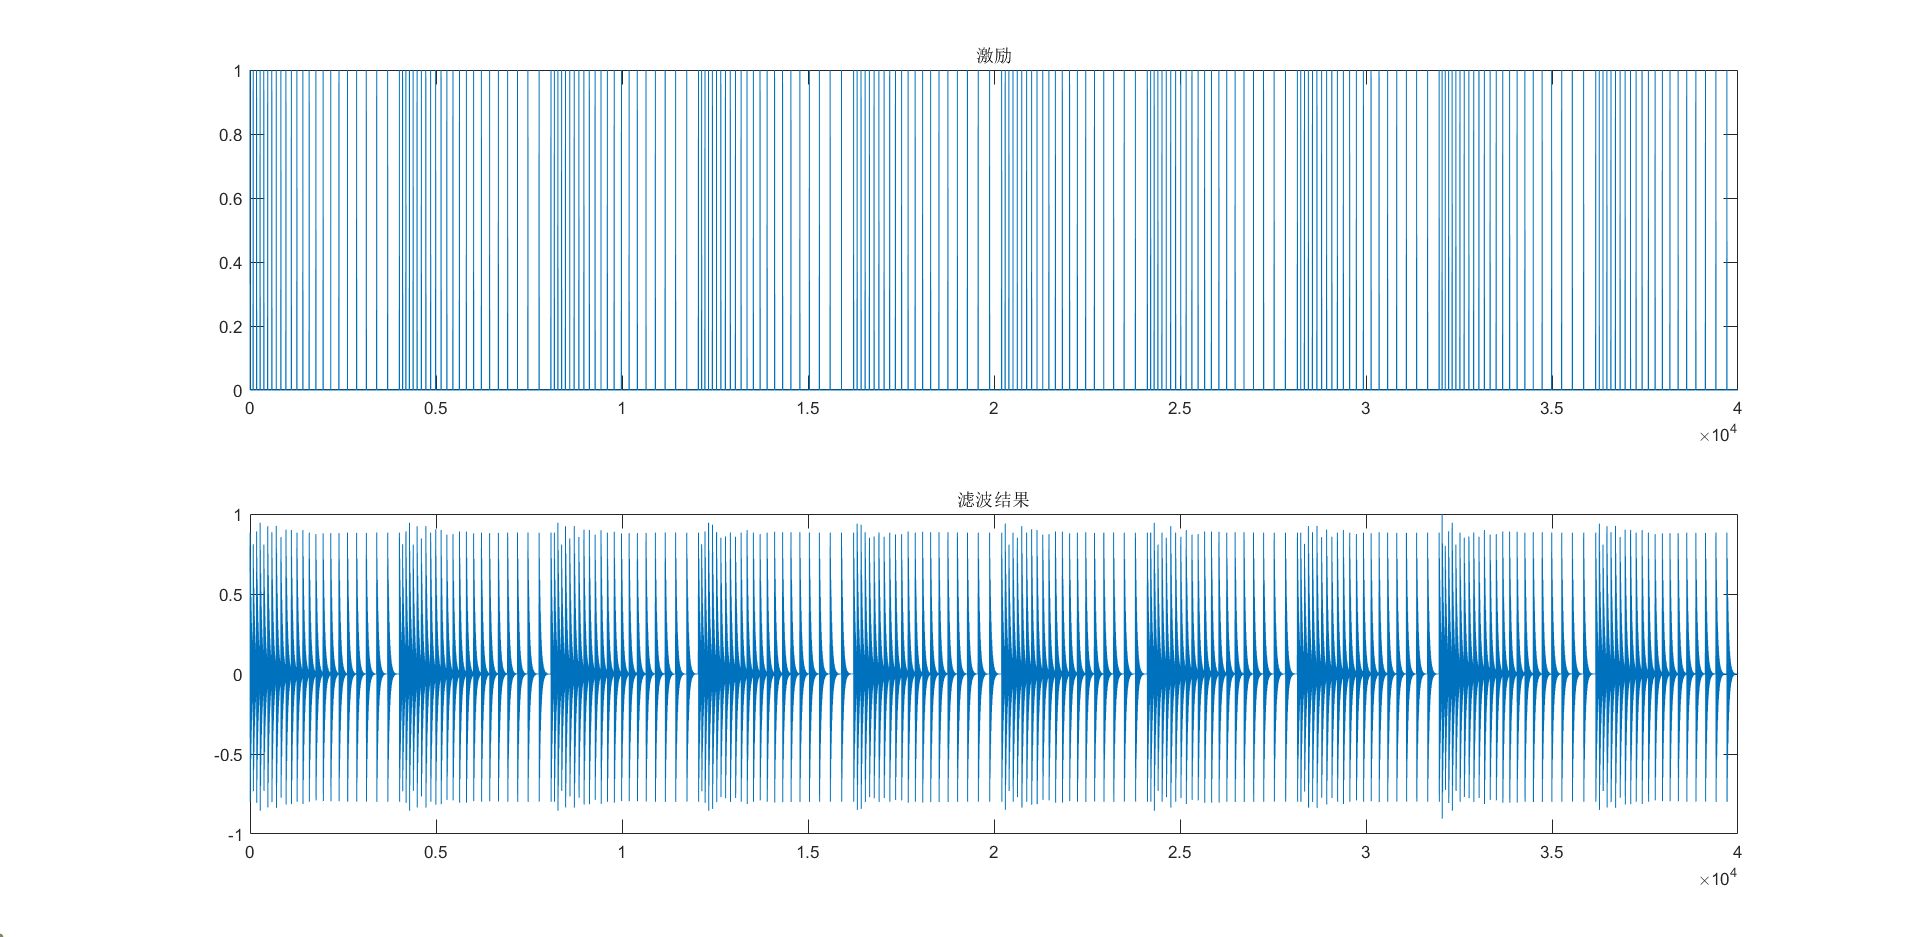
\includegraphics[width=.8\textwidth]{../assets/2_3_time.png}
    \caption{基音周期改变激励及滤波结果时域波形}
    \label{fig:2_3_time}
\end{figure}

\begin{figure}[h]
    \centering
    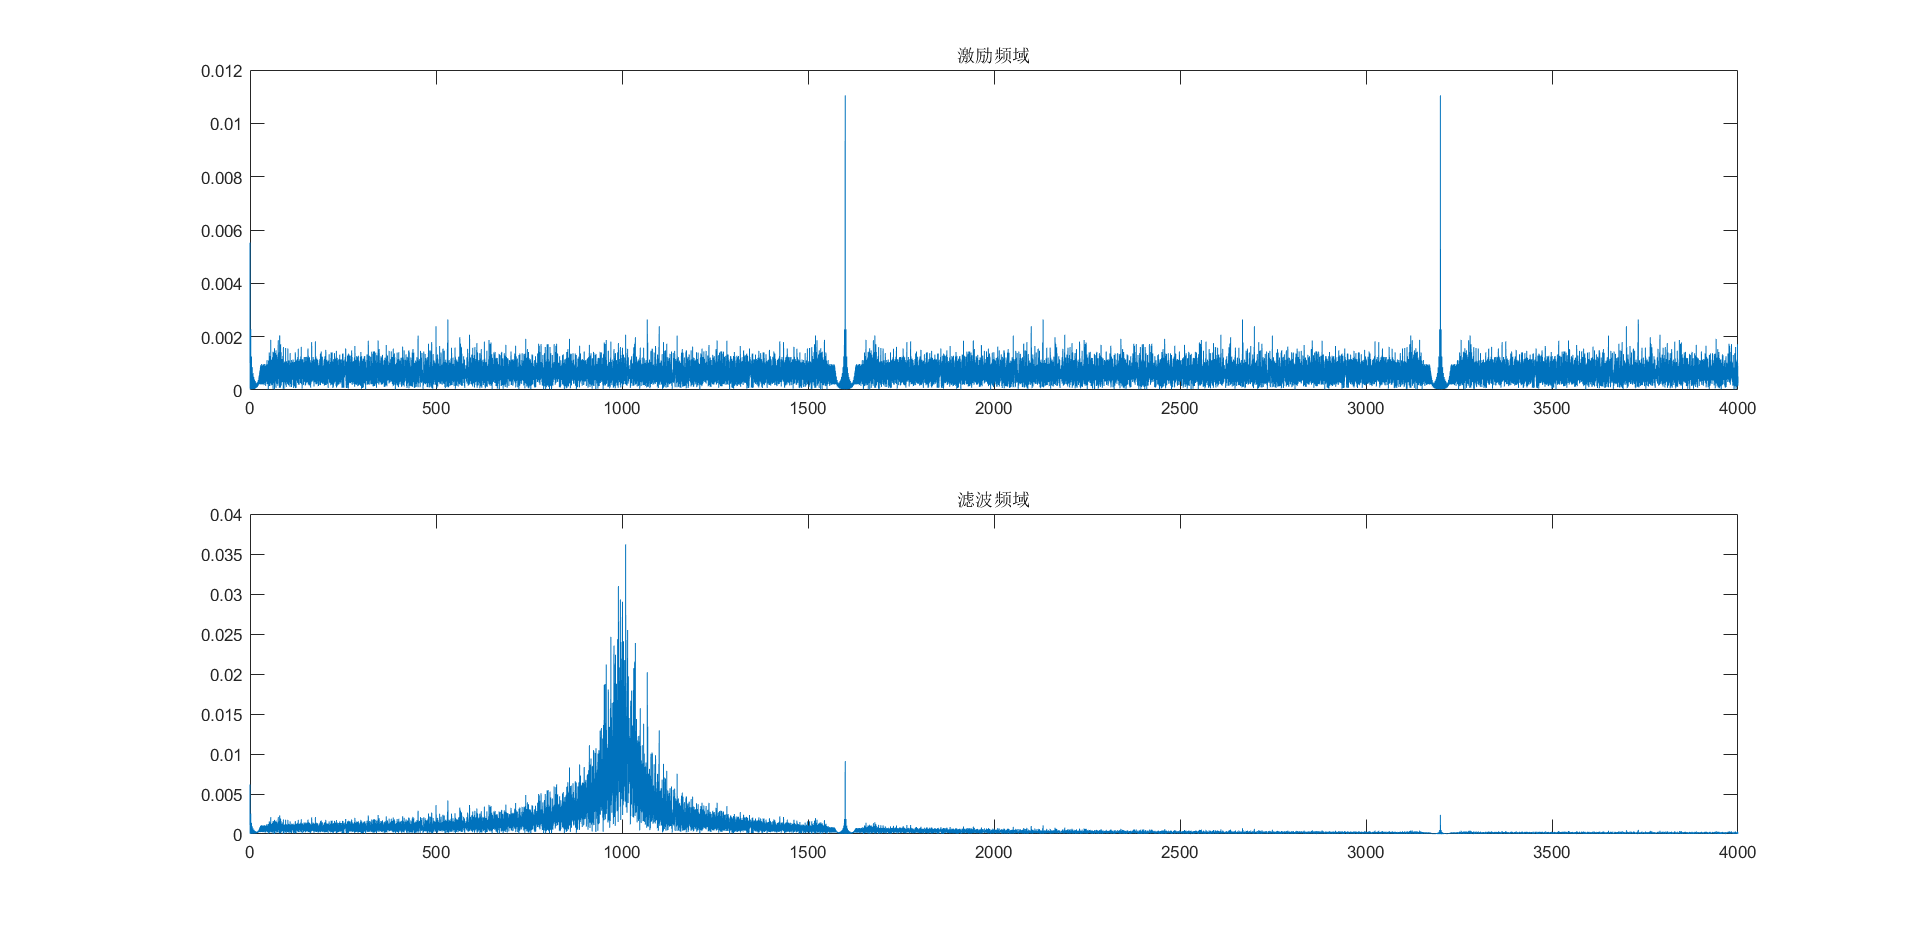
\includegraphics[width=.8\textwidth]{../assets/2_3_freq.png}
    \caption{基音周期改变激励及滤波结果频域波形}
    \label{fig:2_3_freq}
\end{figure}

可以看到,滤波将能量集中到1000Hz附近,增强了低频,与听的结果一致。注意到1000Hz为该滤波器的共振峰频率,符合该滤波器的幅频响应。时域上看是叠加了一个周期性指数衰减的包络,可能因此感觉不那么刺耳。

\subsection{激励、语音合成}\label{sec:syn}

仿照前面章节\mintinline{matlab}{filter}的使用,定义滤波器状态\mintinline{matlab}{zi_syn},并使用下方代码生成激励和重建语音:

\begin{minted}[bgcolor=bg]{matlab}
zi_syn = zeros(P, 1);

pos = (n - 1) * FL + 1;
while pos <= n * FL
    exc_syn(pos) = G;
    pos = pos + PT;
end
[s_syn((n - 1) * FL + 1 : n * FL), zi_syn] = ...
    filter(1, A, exc_syn((n - 1) * FL + 1 : n * FL), zi_syn);
\end{minted}

绘制重建语音和原语音的时域如图\ref{fig:2_4_time},频域如图\ref{fig:2_4_freq}。可以看到,重建语音的能量更集中于一系列频点上,或许失去了一些细节。

听上去,重建语音较类似于老电影中机器人说话的声音,其中“灯”和“进”的音调似乎略有上升,并且接近于中文的“阳平”。

\begin{figure}[h]
    \centering
    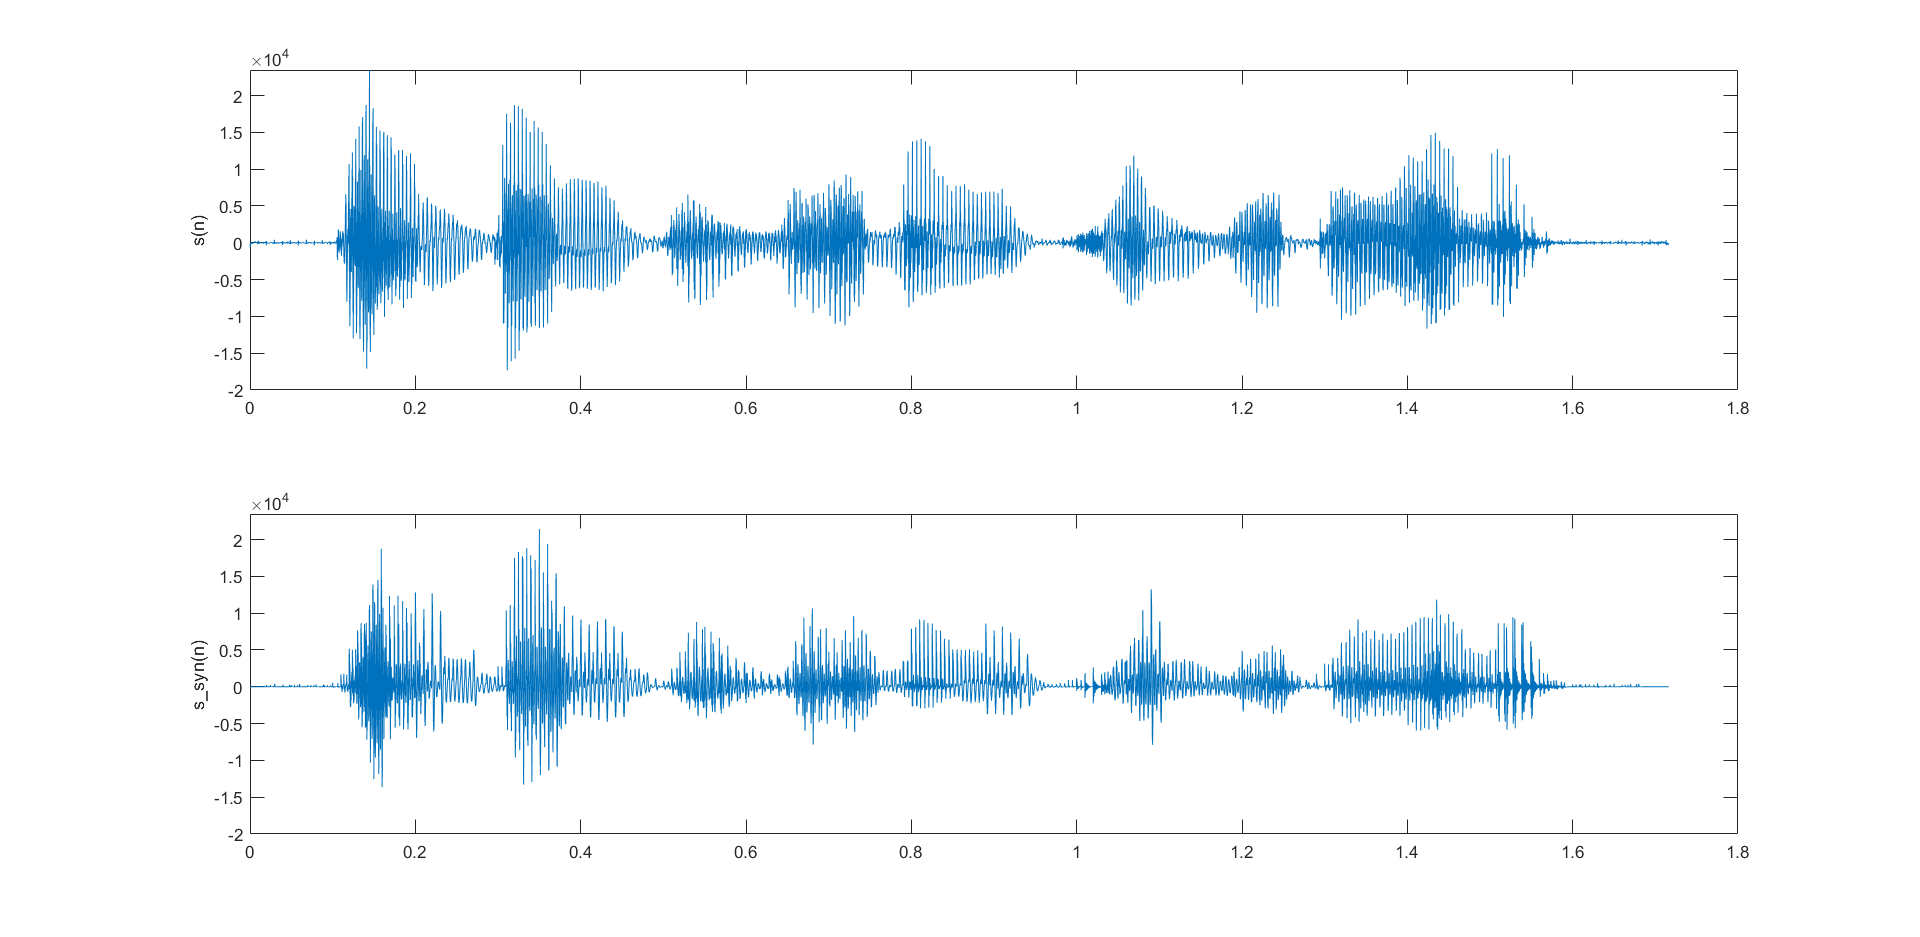
\includegraphics[width=.8\textwidth]{../assets/2_4_time.png}
    \caption{语音和重建语音时域波形}
    \label{fig:2_4_time}
\end{figure}

\begin{figure}[h]
    \centering
    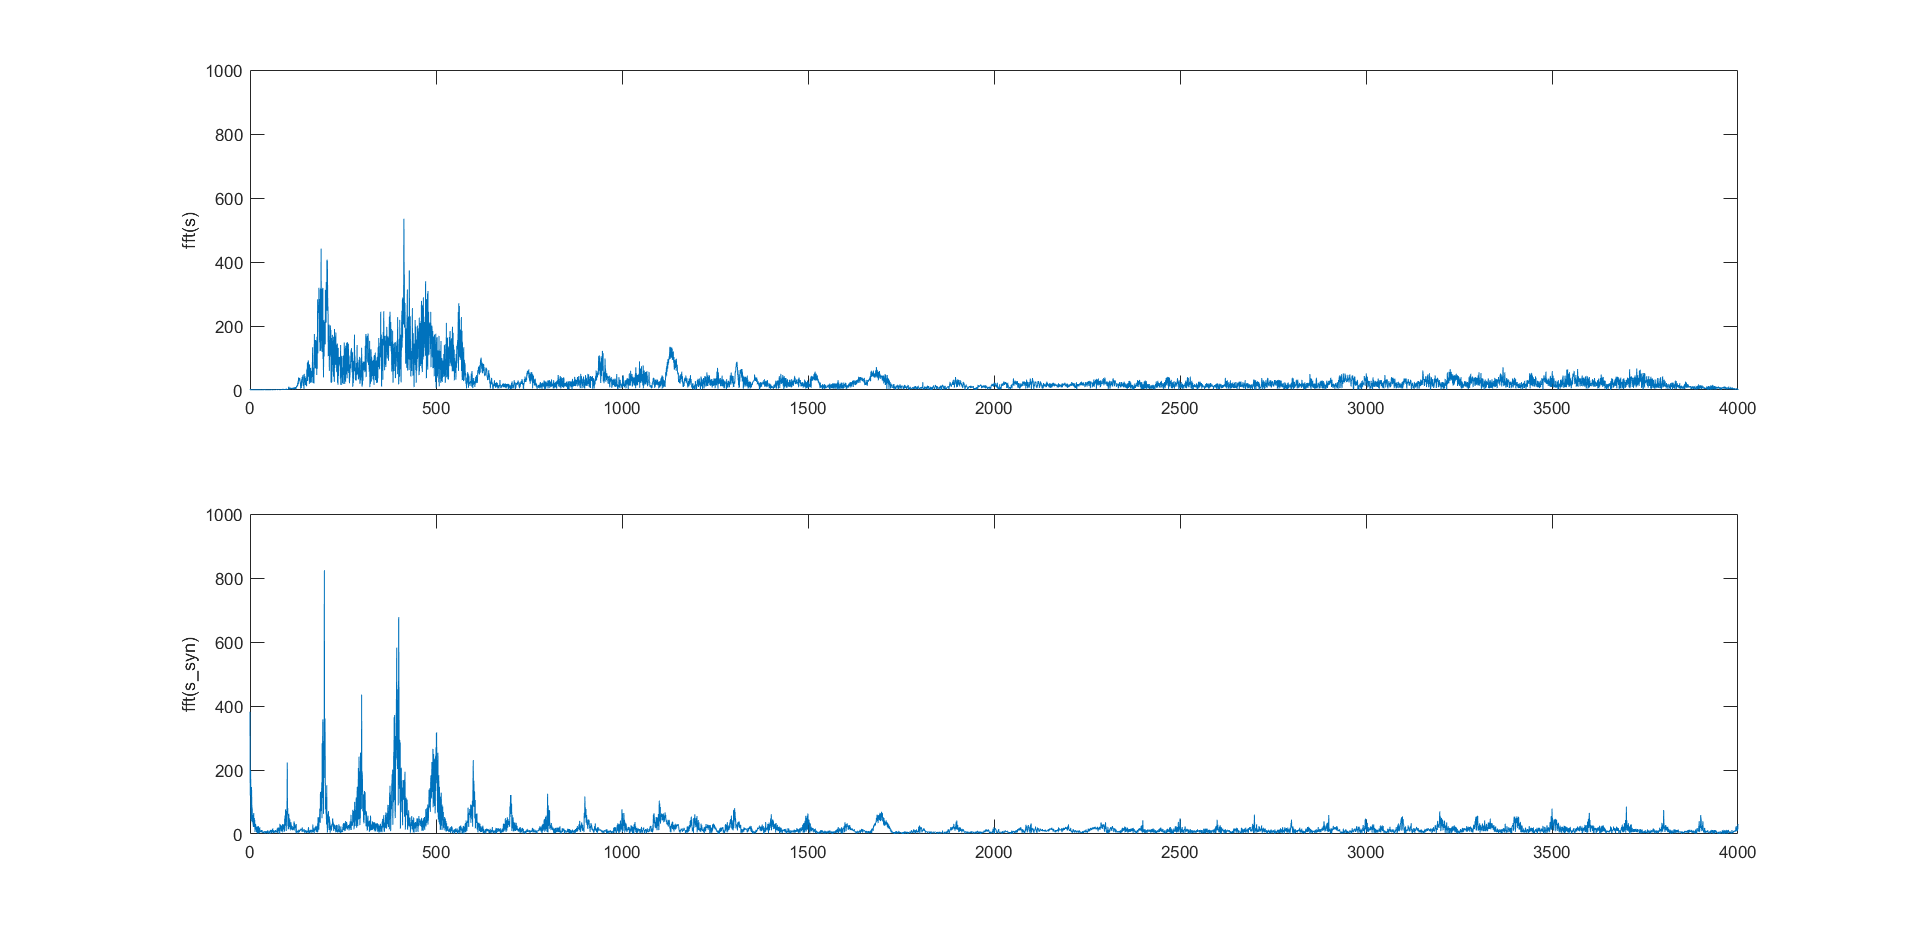
\includegraphics[width=.8\textwidth]{../assets/2_4_freq.png}
    \caption{语音和重建语音频域波形}
    \label{fig:2_4_freq}
\end{figure}

\section{变速不变调}

\subsection{激励长度翻倍的语音合成}

与节\ref{sec:syn}类似,定义滤波器状态、生成激励并重建语音。代码如下:

\begin{minted}[bgcolor=bg]{matlab}
zi_syn_v = zeros(P, 1);

FL_v = FL * 2;
pos_v = (n - 1) * FL_v + 1;
while pos_v <= n * FL_v
    exc_syn_v(pos_v) = G;
    pos_v = pos_v + PT;
end
[s_syn_v((n - 1) * FL_v + 1 : n * FL_v), zi_syn_v] = ...
    filter(1, A, exc_syn_v((n - 1) * FL_v + 1 : n * FL_v), zi_syn_v);
\end{minted}

听上去音调没有变化,而速度变慢了一倍,可以清晰地听到语音中的“颗粒感”,更加类似老电影中机器人说话的声音。

\section{变调不变速}

\subsection{共振峰频率提高150Hz的\ref{sec:filter}滤波器}

回顾节\ref{sec:filter}中共振峰频率的计算,只需将共轭极点的辐角绝对值增大,便可以提高共振峰频率。欲求新的极点,可以通过乘以$e^{\pm i\theta}$来改变辐角。下面使用代码求解:

\begin{minted}[bgcolor=bg]{matlab}
b = 1;
a = [1, -1.3789, 0.9506];

rot_angle = 150 * 2 * pi / 8000;

[z, p, k] = tf2zpk(b, a);
p = p .* exp(1i * sign(imag(p)) * rot_angle);

[b, a] = zp2tf(z, p, k);
\end{minted}

求得$a_1 = -1.207283861048186$,$a_2 = 0.950600000000000$。将系数放入节\ref{sec:filter}的代码,得到相关图形。

\begin{figure}[h]
    \centering
    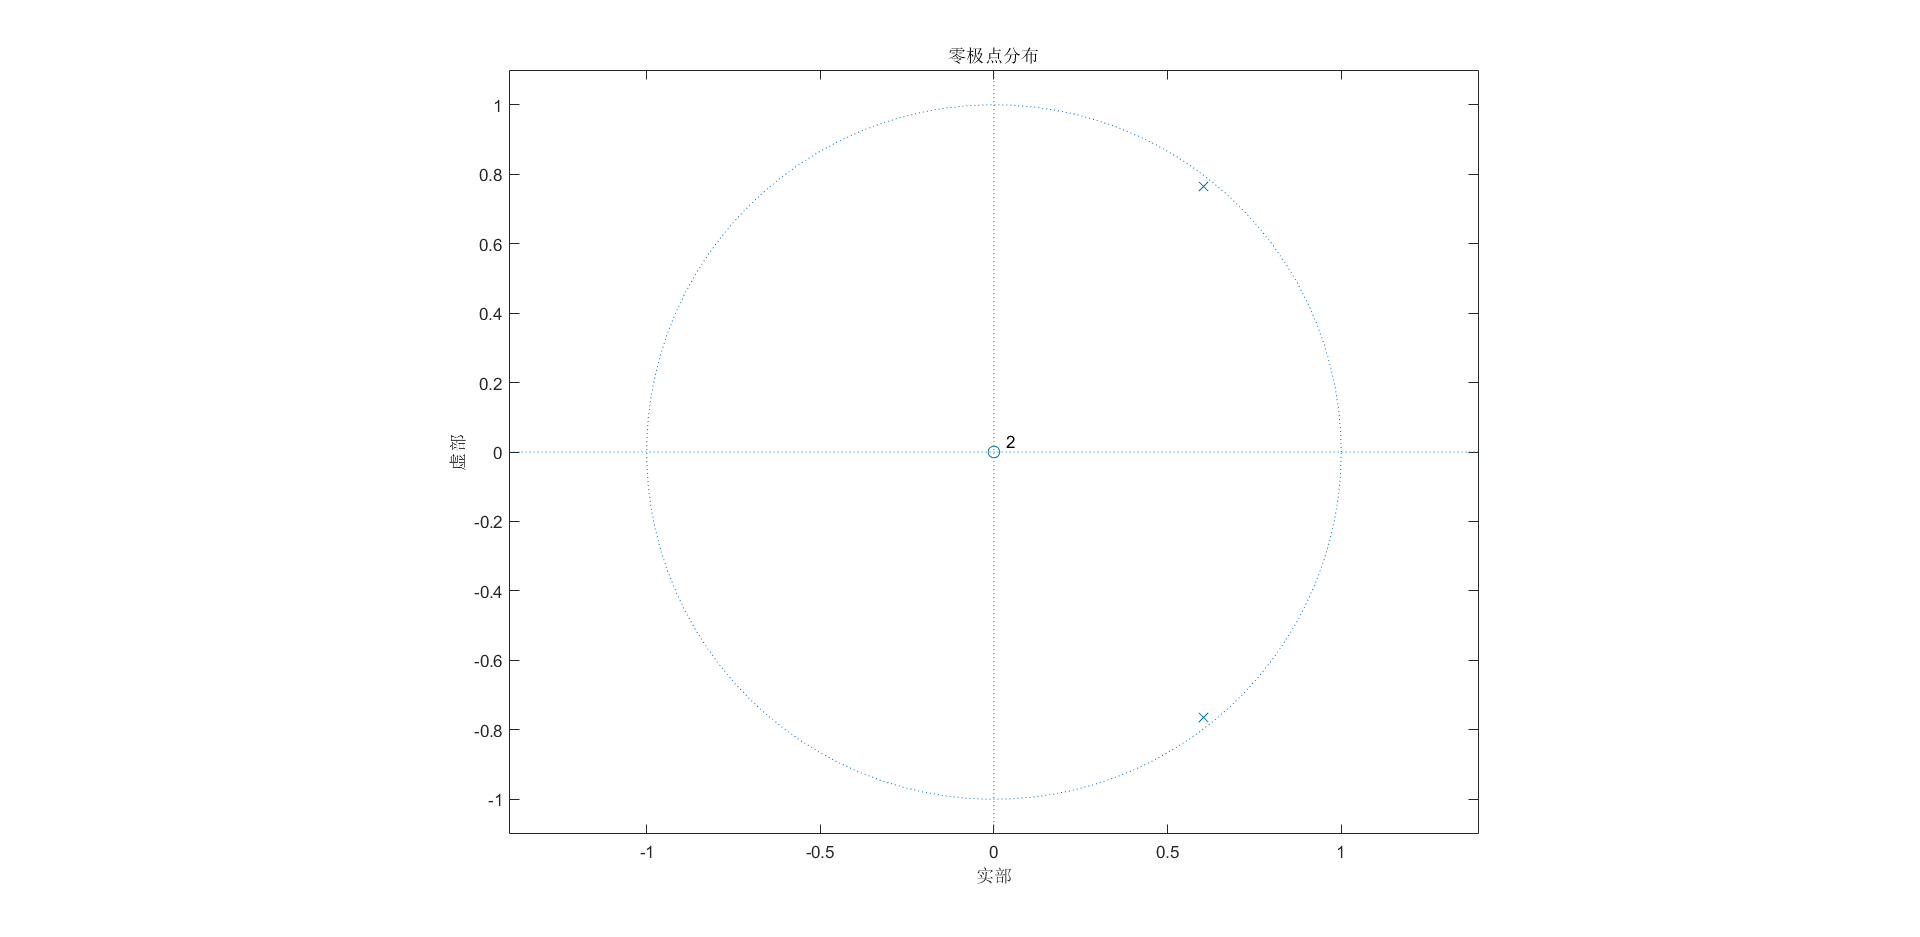
\includegraphics[width=.8\textwidth]{../assets/4_1_zplane.png}
    \caption{共振峰频率增加150Hz的滤波器的零极点分布}
    \label{fig:exp4_1_zplane}
\end{figure}

\begin{figure}[h]
    \centering
    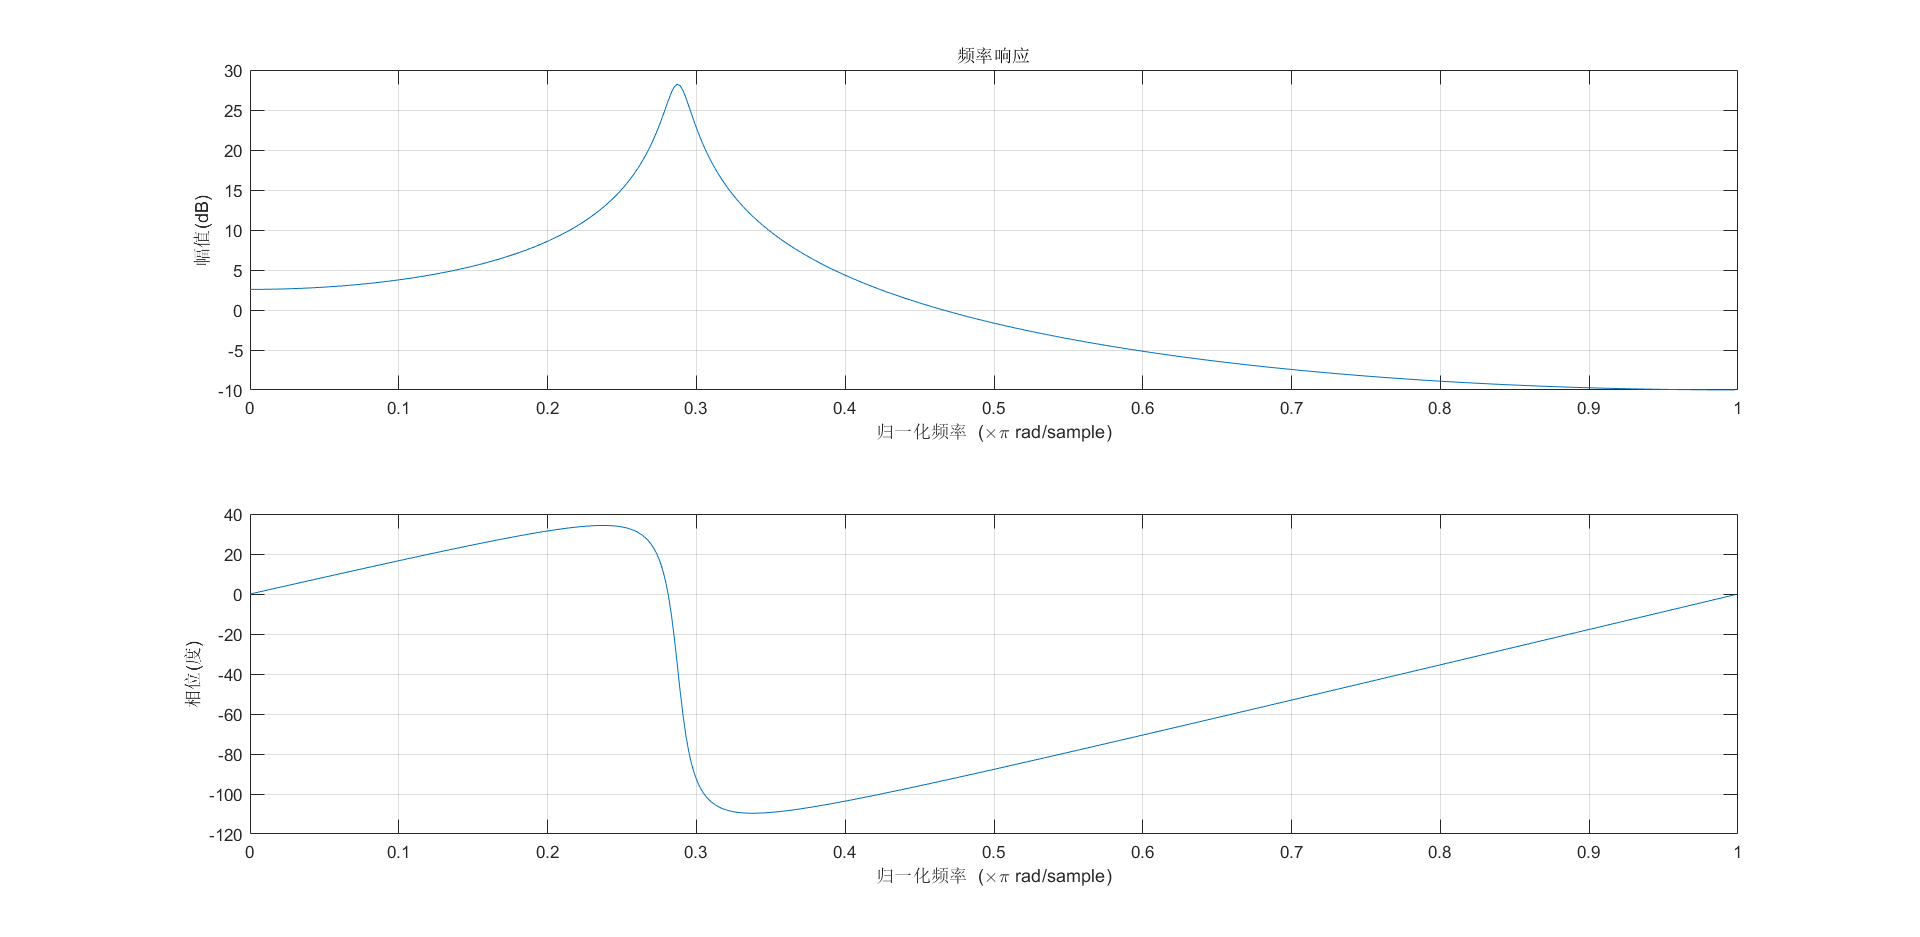
\includegraphics[width=.8\textwidth]{../assets/4_1_freqz.png}
    \caption{共振峰频率增加150Hz的滤波器的频率响应}
    \label{fig:exp4_1_freqz}
\end{figure}

\begin{figure}[!ht]
    \centering
    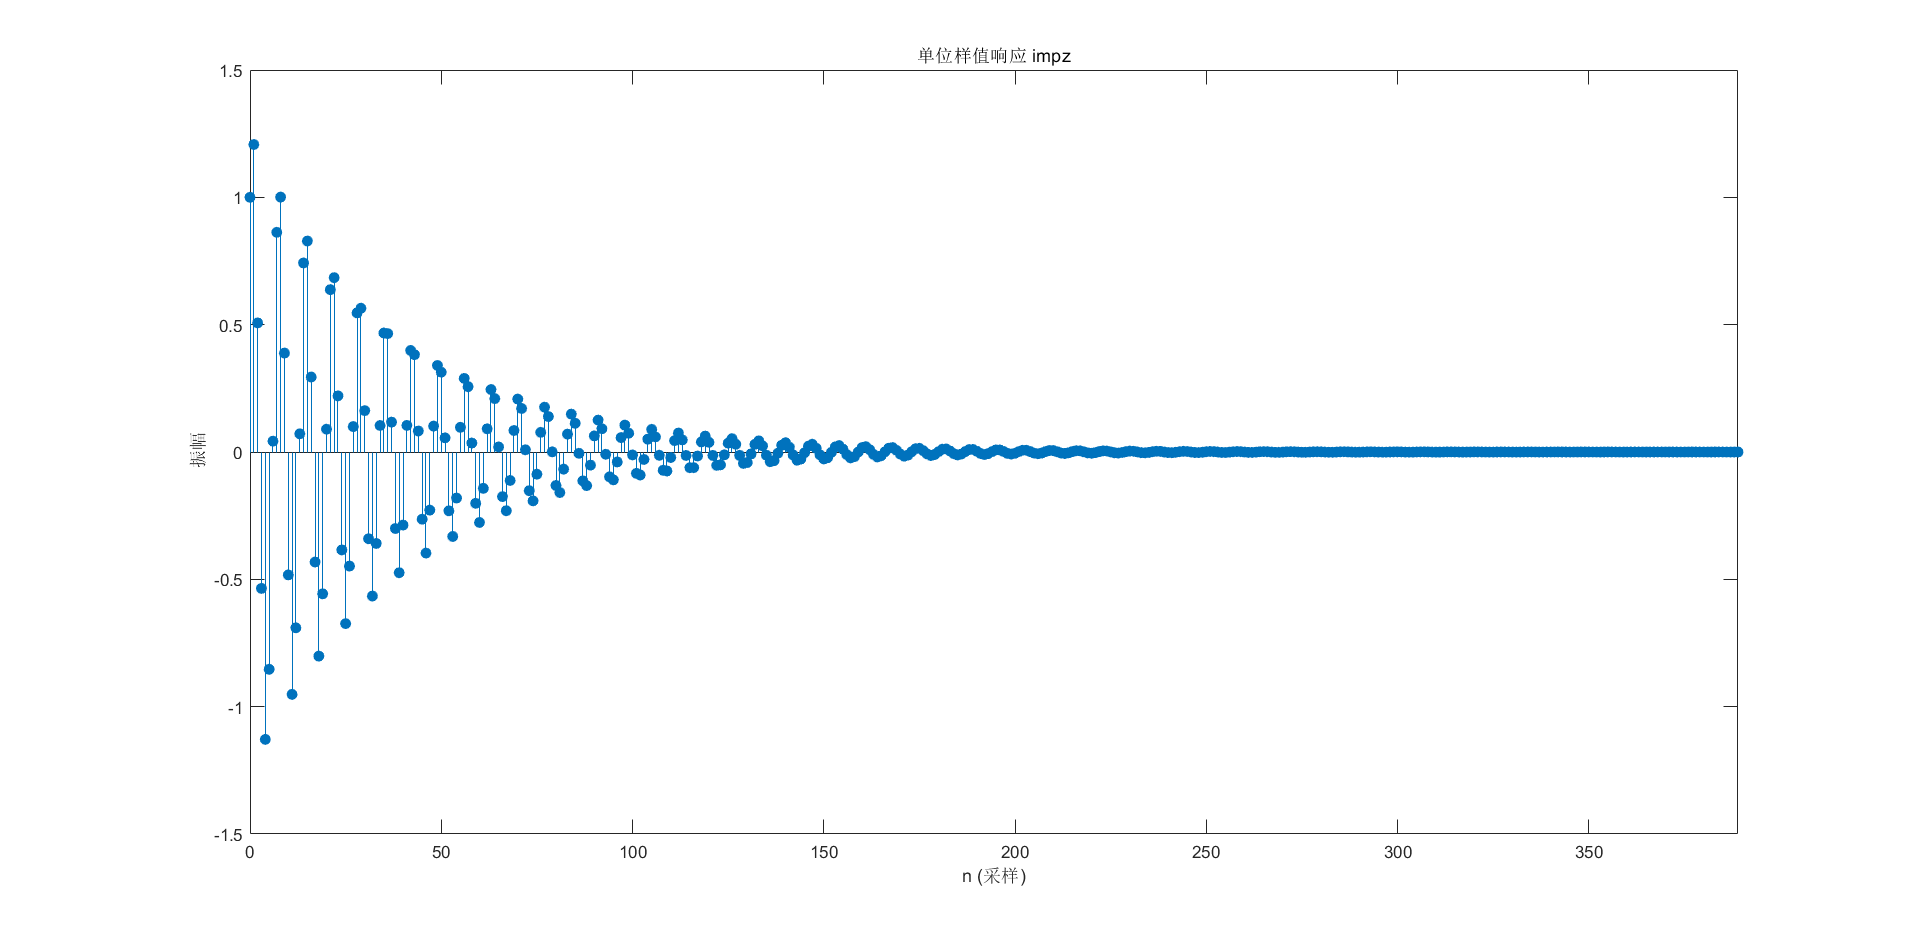
\includegraphics[width=.8\textwidth]{../assets/4_1_impz.png}
    \caption{共振峰频率增加150Hz的滤波器的单位样值响应}
    \label{fig:exp4_1_impz}
\end{figure}

由于极点只变化了约0.12rad,难以从图\ref{fig:exp4_1_zplane}中看出变化。1150Hz对应0.$2875\pi$rad,与图\ref{fig:exp4_1_freqz}一致。注意到图\ref{fig:exp4_1_impz}表现出来的单位样值响应没有\ref{fig:exp1_1_impz}对称,而是错落有致,这应与后面变调的语音合成有关。

\subsection{减半基音周期并提高共振峰频率的语音合成}

与前面实验类似,使用如下代码实现此功能:

\begin{minted}[bgcolor=bg]{matlab}
zi_syn_t = zeros(P, 1);

[z, p, k] = tf2zpk(1, A);
rot_angle = 150 * 2 * pi / 8000;
p = p .* exp(1i * sign(imag(p)) * rot_angle);
[~, A_t] = zp2tf(z, p, k);
pos_t = (n - 1) * FL + 1;
while pos_t <= n * FL
    exc_syn_t(pos_t) = G;
    pos_t = pos_t + round(PT / 2);
end
[s_syn_t((n - 1) * FL + 1 : n * FL), zi_syn_t] = ...
    filter(1, A_t, exc_syn_t((n - 1) * FL + 1 : n * FL), zi_syn_t);
\end{minted}

听上去音调有了显著的上升,更尖,而速度并未变化,与原语音时长一致。

绘制变速和变调的语音波形,时域见图\ref{fig:4_2_time},频域见图\ref{fig:4_2_freq}。

\begin{figure}[!ht]
    \centering
    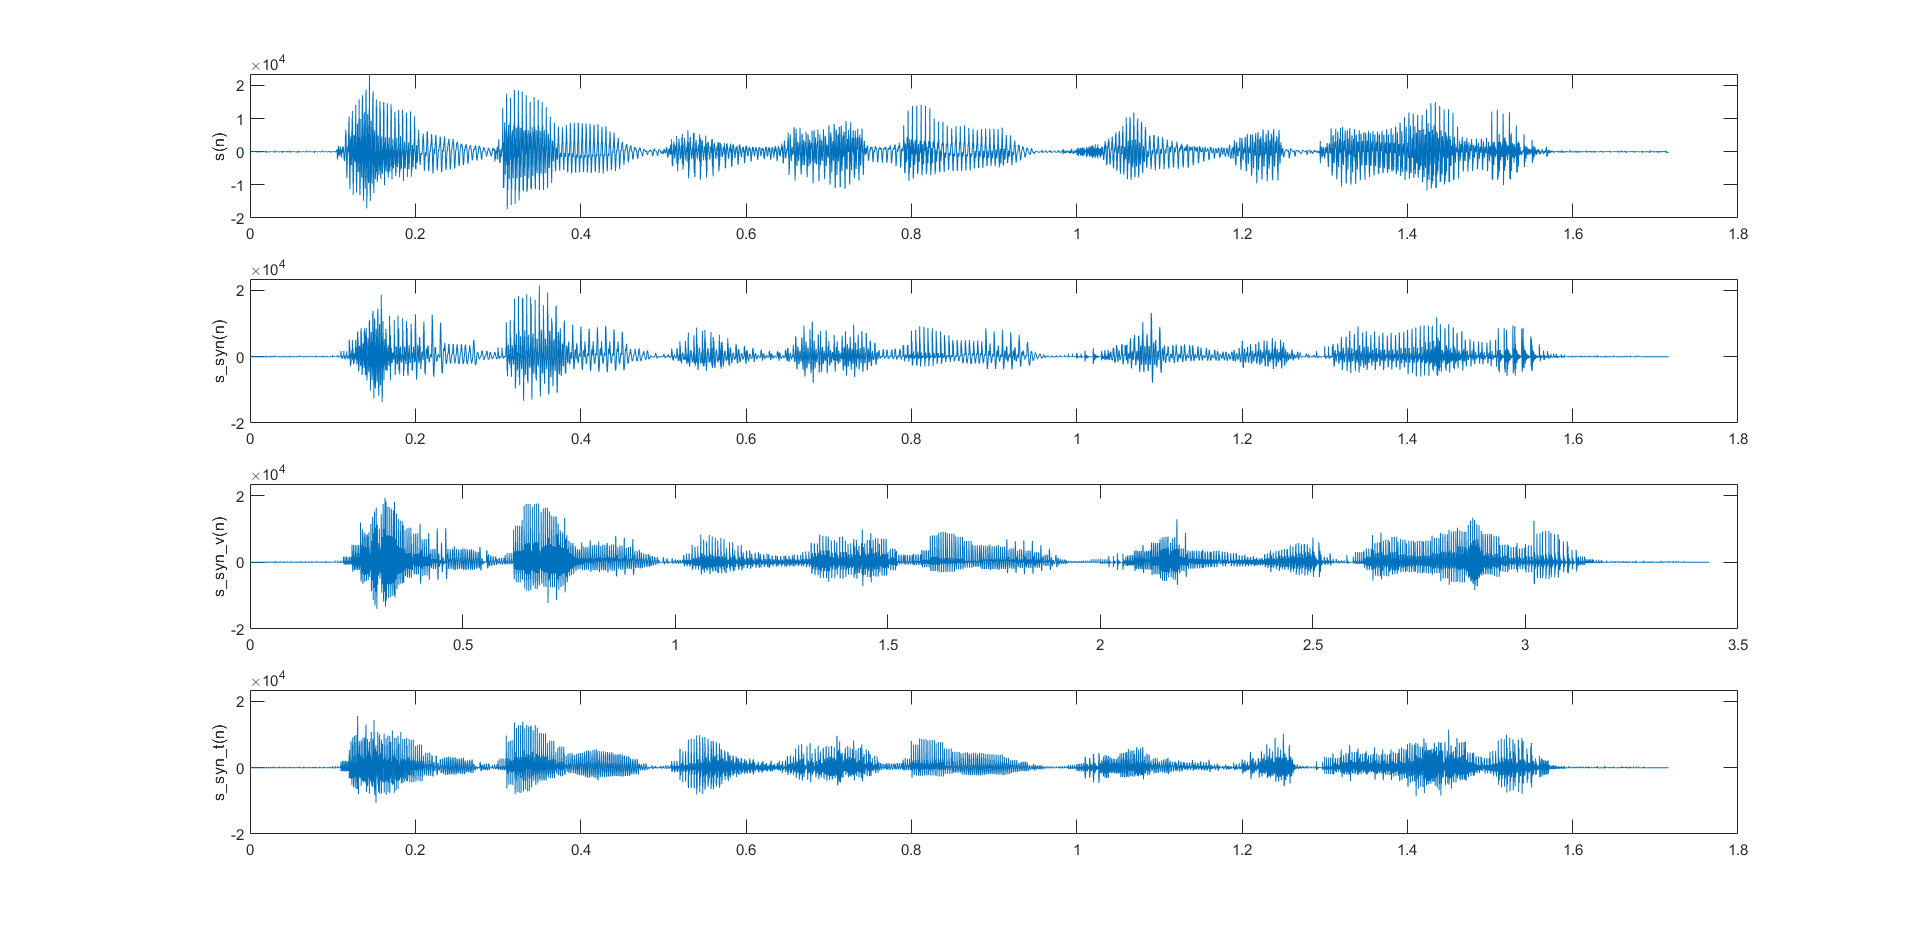
\includegraphics[width=.8\textwidth]{../assets/4_2_time.png}
    \caption{重建语音时域波形}
    \label{fig:4_2_time}
\end{figure}

\begin{figure}[!ht]
    \centering
    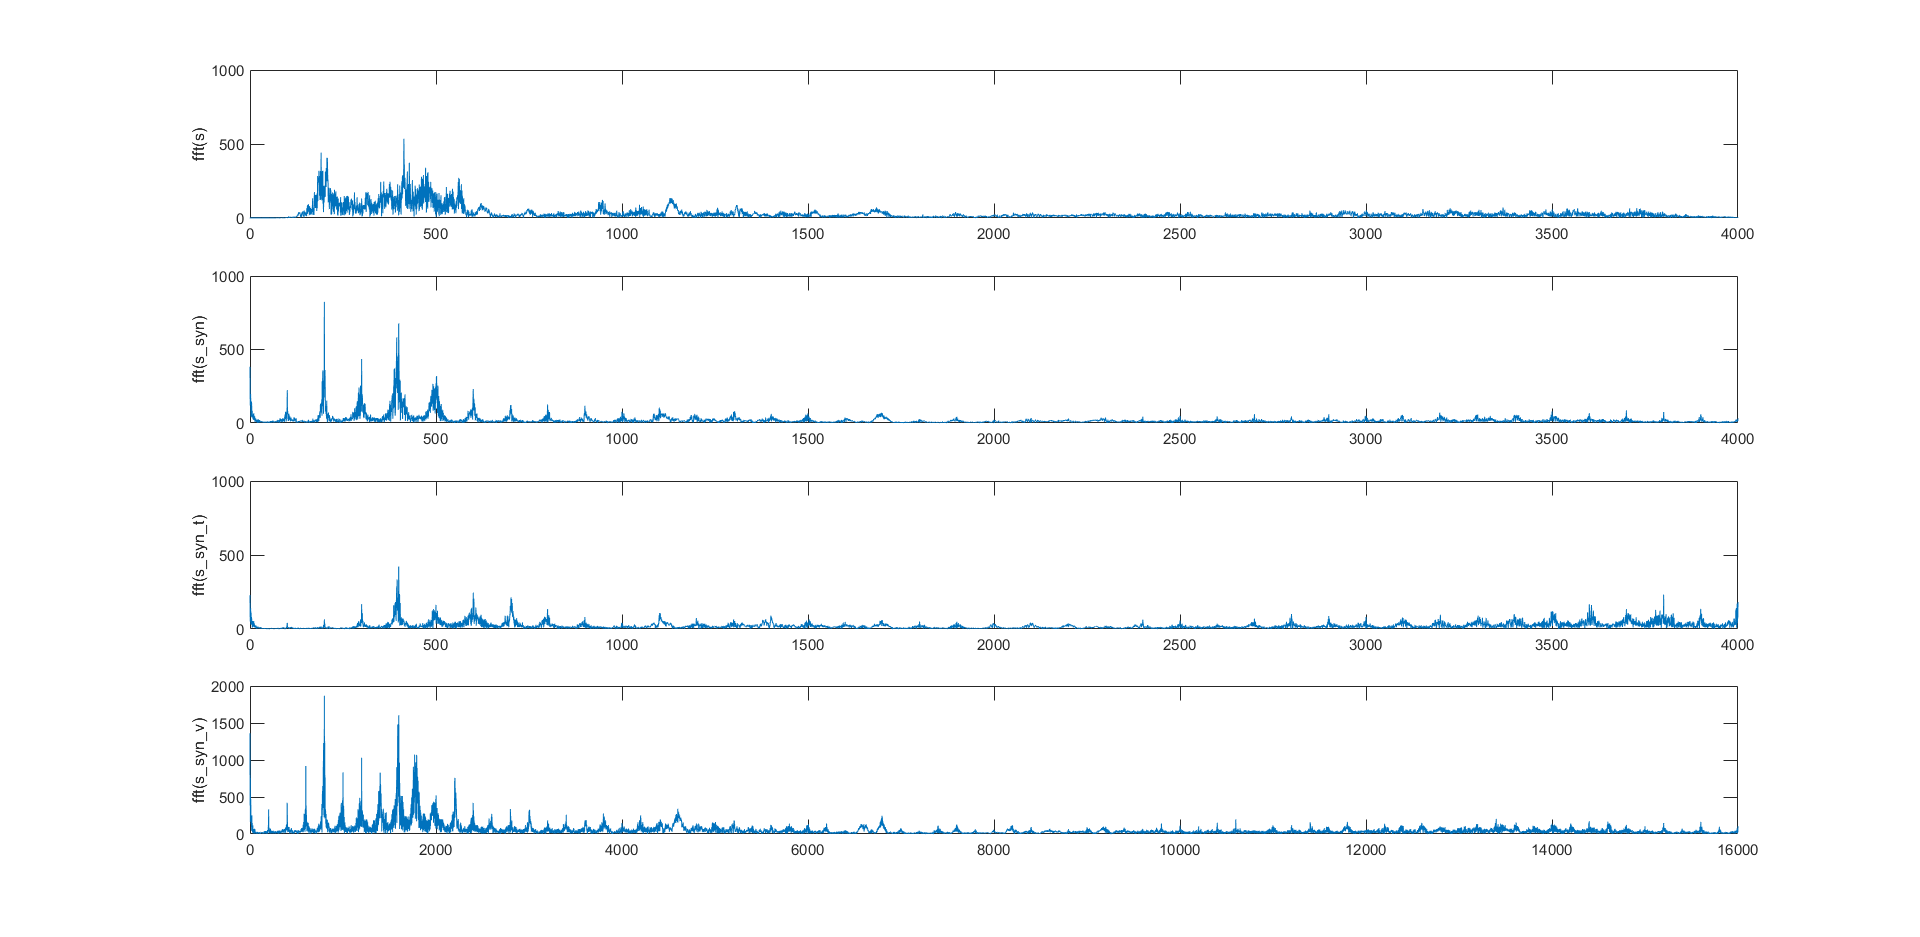
\includegraphics[width=.8\textwidth]{../assets/4_2_freq.png}
    \caption{重建语音频域波形}
    \label{fig:4_2_freq}
\end{figure}

从图\ref{fig:4_2_time}可以直观地看出变数不变调虽然时长变为了两倍,但波形基本没有变化,这与听上去音调没有变化是相符的。而变调不变速则是时长没有变化,但波形显得更为密集,且形状发生了改变,这也与听上去的感受相符。图\ref{fig:4_2_freq}显示出变调不变速明显将能量向高频移动了。值得注意的是,变数不变调的频谱中也有较多高频分量,我认为这是由于激励长度翻倍的处理中引入的高频分量,表现在听的感受上是一些类似“颤音”的背景声。而人耳听起来并不是语音的主要特征,故感受上整体音调是没有变化的。

\section{后记}

\end{document}